\documentclass[12pt, A4]{article}
\usepackage[top=1in,left=1in,bottom=1in,right=1in]{geometry}


%Packages
\usepackage{sectsty}
\usepackage[hyphens]{url}
\usepackage[breaklinks]{hyperref}
\usepackage{amsmath, amssymb, amsthm, amsbsy, amsfonts, cases}
\usepackage{graphicx, comment, enumitem}
\usepackage{algorithm, algcompatible}
\usepackage[noend]{algpseudocode}
\sectionfont{\fontsize{14}{14}\selectfont}
\subsectionfont{\fontsize{12}{12}\selectfont}
\usepackage{bigints}
\usepackage[mathscr]{euscript}
\usepackage[makeroom]{cancel}
\usepackage{graphicx}
\usepackage[table]{xcolor}
\usepackage{subcaption}
\usepackage{enumerate, verbatim}
\usepackage[font={small,it,singlespacing}]{caption}
\usepackage{lscape}
%\usepackage[nodisplayskipstretch]{setspace}
\usepackage{caption}
\usepackage{hyperref}
\usepackage[sort]{natbib}
\usepackage{parskip}
\usepackage{array}
\usepackage{multirow}
\usepackage{graphicx}
\usepackage{wrapfig}
\usepackage{lscape}
\usepackage{rotating}
\usepackage{epstopdf}
\usepackage[compact]{titlesec}

\usepackage{color, colortbl, setspace}
\definecolor{Gray}{gray}{0.9}

\usepackage{boldline}
%Margins
% \setlength{\topmargin}{-0.5in}
% \setlength{\textheight}{9in}
% \setlength{\oddsidemargin}{-0.3in}
% \setlength{\textwidth}{7.2in}
\hypersetup{colorlinks,citecolor=blue}
\setlength{\parindent}{.3in}
\graphicspath{{./images//}}

\setlength{\abovedisplayskip}{3pt}
\setlength{\belowdisplayskip}{3pt}
%\setlength{\abovedisplayshortskip}{-6pt}
%\setlength{\belowdisplayshortskip}{-6pt}
\setlength{\belowcaptionskip}{-3pt}

\renewcommand*{\thefootnote}{\arabic{footnote}}
\renewcommand{\qedsymbol}{$\blacksquare$}
\newcommand{\bs}{\boldsymbol}
\newcommand{\R}{\mathcal{R}}
\newcommand{\T}{\mathcal{T}}
\newcommand{\x}{\mathbf{x}}
\newcommand{\z}{\mathbf{z}}
\newcommand{\w}{\mathbf{w}}
\newcommand{\s}{\mathbf{s}}
\newcommand{\e}{\mathbf{e}}
\newcommand{\vv}{\mathbf{v}}
\newcommand{\Lap}{\mathcal{LAP}}
\newcommand{\Exp}{\mathcal{EXP}}
\newcommand{\E}{\mbox{E}}

\newcolumntype{L}[1]{>{\raggedright\let\newline\\\arraybackslash\hspace{0pt}}m{#1}}
\newcolumntype{C}[1]{>{\centering\let\newline\\\arraybackslash\hspace{0pt}}m{#1}}
\newcolumntype{R}[1]{>{\raggedleft\let\newline\\\arraybackslash\hspace{0pt}}m{#1}}

%\theoremstyle{definition}
\theoremstyle{plain}
\newtheorem{thm}{Theorem}%[section]
%\newtheorem{defn}{Definition}[section]
\newtheoremstyle{exampstyle}
  {6pt} % Space above
  {\topsep} % Space below
  {} % Body font
  {} % Indent amount
  {\bfseries} % Theorem head font
  {.} % Punctuation after theorem head
  {.5em} % Space after theorem head
  {} % Theorem head spec (can be left empty, meaning `normal')
\theoremstyle{exampstyle}\newtheorem{defn}{Definition}
\theoremstyle{exampstyle}\newtheorem{lem}{Lemma}
\theoremstyle{exampstyle}\newtheorem{cor}{Corollary}
\theoremstyle{exampstyle}\newtheorem{pro}{Proposition}
\theoremstyle{exampstyle}\newtheorem{cla}{Claim}
\theoremstyle{exampstyle}\newtheorem{rem}{Remark}

\newcommand{\beginsupplement}{%
        \setcounter{table}{0}
        \renewcommand{\thetable}{S\arabic{table}}%
        \setcounter{figure}{0}
        \renewcommand{\thefigure}{S\arabic{figure}}%
}

\setlength{\parskip}{6pt}
\setlength\parindent{0pt}
\titlespacing*{\section}{0pt}{3pt}{3pt}
\titlespacing*{\subsection}{0pt}{3pt}{3pt}

\begin{document}
\title{\large{\textbf{Differentially Private Data Release via\\ Statistical Election to Partition Sequentially}}}
\author{\small{\textbf{Claire McKay Bowen, Fang Liu, Bingyue Su}}
\footnote{\noindent Claire McKay Bowen is the Lead Data Scientist for Privacy and Data Security at the Urban Institute. Fang Liu is an Associate Professor and Bingyue Su is a doctoral student in the Department of Applied and Computational Mathematics and Statistics, University of Notre Dame, Notre Dame, IN 46556. Claire McKay Bowen was supported by the National Science Foundation (NSF) Graduate Research Fellowship under Grant No. DGE-1313583 during part of the development of this paper. Fang Liu was supported by the NSF Grants  \#1546373, \#1717417, and the University of Notre Dame Faculty Research Support Initiation Grant Program. Bingyue Su is supported by the NSF Grant \#1717417.} 
\vspace{-3.5cm}
}
\date{}
\maketitle{}

\begin{abstract}
\noindent Differential Privacy (DP) formalizes privacy in rigorous and mathematical terms as well as provides a robust concept for privacy protection. DIfferentially Private Data Synthesis (DIPS) techniques produce and release synthetic individual-level data based on the DP framework. However, statistical utility of the synthetic data via DIPS can be low due to the potentially large amount of noise injected to satisfy DP, especially in high-dimensional data. We propose a new DIPS approach, STatistical Election to Partition Sequentially (STEPS), that partitions data by attributes according to their importance ranks per either a practical importance or statistical importance measure. The higher the rank is for an attribute, the better the original information is preserved for that attribute in the synthetic data, and the more useful the synthetic data are expected to be, overall. We develop a general-utility metric to assess the similarity of the synthetic data to the actual data. We applied the STEPS procedure to both simulated data and the 2000-2012 Current Population Survey youth voter data. The results suggest STEPS can preserve better the population-level information and the original information for some analyses compared to the PrivBayes, a modified Uniform histogram approach, and the flat Laplace sanitizer.\\

\noindent \textit{\textbf{keywords}}:  privacy budget, DIfferentially Private Data Synthesis (DIPS), statistical disclosure limitation, propensity score, universal histogram
\end{abstract}

%%%%%%%%%%%%%%%%%%%%%%%%%%%%%%%%%%%%%%%%%%%%%%%%%%%%%%%%%%%%%%%%%%%%%%%%%%%%%%%%
% Intro
%%%%%%%%%%%%%%%%%%%%%%%%%%%%%%%%%%%%%%%%%%%%%%%%%%%%%%%%%%%%%%%%%%%%%%%%%%%%%%%%
\newpage
\setstretch{1.05}
\section{Introduction}\label{sec:intro}

Data privacy protection techniques are often referred to as the statistical disclosure limitation or control in the statistical community. Various approaches have been developed to provide protection for individual sensitive information when releasing data to researchers or the public. Among these approaches, data synthesis is a popular technique that generates synthetic individual-level data given the original data \citep{rubin1993discussion, little1993statistical, liu2003,raghunathan2003multiple, reiter2003,  liu2004, reiter2009, drechsler2011book}. The synthetic data approach is appealing as it provides surrogate data that have the same structure as the original data, but sanitized for privacy and users may perform their own analyses as if they had the original data. A line of research to generate synthetic data with a preset privacy risk level is DIfferentially Private data Synthesis (DIPS). DIPS combines data synthesis with differential privacy (DP), a rigorous mathematical framework that controls privacy risk with a prespecified privacy budget  \citep{dwork2006calibrating}. Interested readers are referred to \citet{bowen2016differentially} for comparisons of several DIPS approaches on the statistical utility of the synthetic data generated by them. Some DIPS methods are ``flat'' or one-step in the sense that DP noises are injected all at once, such as the smooth and perturbed histograms \citep{wasserman2010statistical}, MOdel-based DIPS (MODIPS) \citep{liu2016model}, DPCopula \citep{DPcopula}, and PrivBayes \citep{privbayes},  among others.  

There also exists DP procedures that use sequential partitioning to improve accuracy of range count queries in the 1D and 2D settings. In other words, the queries that are sanitized are associated with sequentially partitioned data and often have a hierarchical relationship among them. Though the focus of these DP mechanisms is not data synthesis, but to improve accuracy of certain queries on numerical attributes in low-dimensional settings, if the counts in the full-dimensional histogram can be calculated or directly sanitized in the process, synthetic data can be generated. We refer to this type of DIPS as sequential or hierarchical. \citet{xiao2010differentially} proposed Privelet via a two-step wavelet-based multidimensional partitioning approach to release range count queries. Privelet has been shown to be effective in the one-dimensional case, but makes only slight improvements in the two-dimensional case, and the performance could be even worse at higher dimensions \citep{qardaji2013geo}. \citet{xiao2012dpcube} presented DPCube as a two-phase partitioning approach for multidimensional data cubes or histograms. \citet{gardner2013share} implemented DPCube in biomedical data to explore its practical feasibility on real-world data sets, but discovered that DPCube is inefficient in constructing accurate high-dimensional histograms. \citet{hay2010boosting} developed the universal histogram to inject noise to histogram bi-partitioning with improved accuracy in histogram bin counts by exploring the inherent consistency constraints. \cite{qardaji2013understanding} extended the method to relatively high dimensional data. \citet{hay2016principled} conducted an extensive comparison on most of the above mentioned algorithms using a set of evaluation principles (DPBench), and provided valuable insights on the pros and cons on the  methods for answering 1- and 2-dimensional range queries. \citet{li2017partitioning} introduced the privacy-aware partitioning mechanism and the utility-based partitioning mechanism that depend on a public but personalized privacy parameter. These methods have not been implemented to real-world data likely due to being ``unable to provide corresponding error guarantees with such procedures for general functions'' \citep{cummings2018individual}. 

While it is possible to directly apply the above hierarchical DP procedures for data synthesis, most of the procedures focus on low dimensional data with numerical attributes. We propose a new DIPS procedure -- \textbf{ST}atistical \textbf{E}lection to \textbf{P}artition \textbf{S}equentially (STEPS), inspired by the hierarchical  DP procedures that sanitizes queries with data partitioning, exploring the potential in improving the utility of the synthetic data in relatively high dimensional settings when the original data have both categorical and numerical attributes. 

STEPS injects noises to a hierarchical histogram. The structure of the histogram is informed either by domain or prior knowledge, or by an information-theoretic metric that explores the inherent statistical information in the original data. Different layers on the same branch in the hierarchical histogram in STEPS contains different attributes, rather than allowing the same attribute to span over multiple layers, which is the case in some of the existing hierarchical DP procedures for releasing queries (e.g., universal histograms). The hierarchical histogram built by STEPS is also subject to equality constraints among the nodes from different layers on the same branch; a post-processing procedure similar to the universal histogram approach \citep{hay2010boosting} will be used to ensure that the equality constraints are satisfied. The final step is to generate synthetic data from the differentially private hierarchical histogram. We expect that STEPS will improve the statistical utility of the released data compared to data synthesized through a random partitioning given that the partitioning in STEPS is an informed decision. We apply STEPS to simulated data and the youth voter data from the 2000-2012 Current Population Survey (CPS) and compare its utility against several commonly used one-step DIPS approach and a modified version of the universal histogram. To assess the similarity of the synthetic data with the original data, we develop a propensity score based method that provides a general utility metric and a holistic measure for the similarity of two data sets of the same structure. 

The remainder of the paper is organized as follows. Section \ref{sec:methodology} provides a brief overview on the preliminaries regarding DP and introduces the STEPS procedure. Section \ref{sec:simulation} applies STEPS to simulated data and compares its capability in preserving the population-level information against PrivBayes and a modified universal histogram procedure. Section \ref{sec:voter} implements the STEPS method to the CPS youth voter data and compares the statistical utility of the synthetic data generated by STEPS with PrivBayes, a modified universal histogram procedure, and a flat Laplace sanitizer via several utility analysis. In Section \ref{sec:disc}, we discuss the implications of our results and provide future research directions.

%%%%%%%%%%%%%%%%%%%%%%%%%%%%%%%%%%%%%%%%%%%%%%
% Statistical Methodology
%%%%%%%%%%%%%%%%%%%%%%%%%%%%%%%%%%%%%%%%%%%%%%%

\section{Methodology}\label{sec:methodology}
\subsection{Preliminaries on Differential Privacy}
DP provides a mathematical and rigorous framework for protecting individual information in a data set, regardless of the background knowledge or behaviors of data intruders, when releasing queries to the public. Query results, in statistical terminology, are statistics; so we will use queries, query results, and statistics, interchangeably, which are denoted by $\s$. We denote the data for privacy protection by $\x=\{x_{ij}\}$ for $i=1,\ldots,n;j=1,\ldots,p$. Each row  $\x_i$ represents an individual record with $p$ variables/attributes. We assume that the sample size $n$ and the number of attributes $p$ are public knowledge and carry no privacy information.
\begin{defn}[\textbf{Differential Privacy} \citep{dwork2006calibrating}]\label{def:dp}
Let $d(\x,\x')=1$ represents all possible ways that data set $\x'$ differing from $\x$ by one individual. A sanitization algorithm $\R$ gives $\epsilon$-DP, if for all data sets $(\x,\x')$ that is $d(\x,\x')=1$ and all result sets $Q\subseteq \T$, where  $\T$ denote the output range of $\R$,  to queries/statistics $\s$ that
\begin{equation}\label{eqn:dp}
\left|\log\left(\frac{\Pr(\R( \s(\x)) \in Q)}{\Pr(\R( \s(\x'))\in Q)} \right)\right|\le\epsilon,
\end{equation}
\noindent where  $\epsilon>0$ is the privacy budget parameter.
\end{defn}
The smaller $\epsilon$ is, the more noises are injected to the statistic $\s$ via the sanitized algorithm $\R$; and each individual in the data set has a lower risk of being identified or having their sensitive information disclosed, because $\s$ would be about the same with and without that individual in the data set. In addition to the $\epsilon$-DP in Definition \ref{def:dp}, there are also  conceptual relaxations of the ``pure'' DP such as the approximate DP \citep{dwork2013algorithmic}, probabilistic DP \citep{machanavajjhala2008privacy}, and concentrated DP \citep{dwork2016concentrated}, among others, so to lessen the amount of noise injected by DP methods by sacrificing a certain amount of privacy.

In regards to what value of $\epsilon$ is considered appropriate or acceptable for practical use, \citet{dwork2008survey} states the choice of $\epsilon$ is a social question. \citet{abowd2015revisiting} acknowledge this and suggest $\epsilon$ at $0.01\sim \ln(3)$, or even up to 3 in releasing certain statistics in social and economic studies. Other $\epsilon$ values have been applied in the literature when DP is applied to cases studies. For instance, \citet{machanavajjhala2008privacy} applied DP in the OnTheMap data (commuting patterns of the United States population) and used $(\epsilon=8.6,\delta=10^{-5})$-probabilistic DP (a relaxation of the pure DP) to synthesize commuter data. \citet{DPcube} and \citet{DPcopula} used $\epsilon=1$. These examples suggest there are many factors that affect the choice of $\epsilon$, including the type of information released to the public, social perception of privacy protection, statistical accuracy of the release data, among others. For a socially acceptable $\epsilon$ given a certain type of information, a differentially private mechanism should aim for maximizing the accuracy of the released information. In other words, choosing an ``appropriate'' $\epsilon$ is essentially a question of finding a good trade-off between privacy loss and released information accuracy.

An important property of DP is that the privacy cost increases for every new query released from the same data set, because more information is ``leaked'' with releasing more query results. Therefore, the data curator must track all statistics calculated on the data set to guarantee the privacy budget does not exceed the prespecified level. For example, if all $q$ queries are sent to data set $\x$, then $\epsilon/q$ can be allocated to each query to ensure the privacy budget is maintained at $\epsilon$ per the \textit{sequential composition} principle \citep{mcsherry2009privacy}. When no overlapping information is requested by different queries, such as when they are calculated from disjoint subsets of a data set, the privacy cost does not accumulate. In such a case, the \textit{parallel composition} principle applies and the overall privacy cost is the maximum privacy budget spent across all the queries \citep{mcsherry2009privacy}.

A common and easy way to implement DP is the Laplace mechanism. A key concept for the Laplace mechanism is the $l_1$ global sensitivity of statistic $\s$ (either a scalar or a vector) is $\Delta_1=\mbox{max}_{\x,\x', d(\x,\x')=1} \|\s(\x)-\s(\x')\|_1$ for all $d(\x,\x')=1$ \citep{dwork2006calibrating}. Global sensitivity can also be defined in other forms, such as the $l_2$ global sensitivity \citep{dwork2013algorithmic} and $l_p$ global sensitivity for any $p\ge1$ \citep{liu2016generalized}.

\begin{defn}[\textbf{Laplace Mechanism} \citep{dwork2006calibrating}]\label{def:lap}
The Laplace sanitizer adds noise to statistics $\s=(s_1,\ldots,s_K)$ via $s_k^\ast=n_k+e_k$, where $e_k{\sim} \text{Lap}(0,\Delta_1/\epsilon)$ and is independent for $k=1,\ldots,K$ and $\Delta_1$ is the $l_1$ global sensitivity of $\s$.
\end{defn}
When $\epsilon$ is small or $\Delta_1$ is large, more Laplace noise is added to $\s$. Other common DP mechanisms include the Gaussian mechanism that is built upon the approximate or the probabilistic DP \citep{dwork2013algorithmic, liu2016generalized}, and the Exponential mechanism that can release both numerical and non-numerical queries \citep{mcsherry2007mechanism}, among others.

\begin{defn}[\textbf{Exponential Mechanism} \citep{mcsherry2007mechanism}]\label{defn:exponential}
Let $u$ be a utility function that assigns a score to each possible output of a query. The exponential mechanism that satisfies $\epsilon$-DP releases query result $s$ calculated from data $D$ with probability  $\exp(u(s)\frac{\epsilon}{2\delta_u})\bigg/\bigintsss_{s'} \exp\!\left(u(s')\frac{\epsilon}{2\delta_u}\right) ds'$, where $\delta_u$ is the maximum change in score $u$ with one element change in data $D$.
\end{defn}


%---------------------------------
\subsection{STatistical Election to Partition Sequentially (STEPS)}\label{sec:steps}

\subsubsection{Overview}
STEPS aims at privately selecting a decomposition sequence  of the joint distribution  of $p$ attributes $\mathbf{X}=(X_1,X_2,\ldots,X_p)$ in the  data, and sanitizing the components in that decomposition according the sequence so to improve the original information preservation on attributes that hold important information and signals for understanding the data.  The outcome of STEPS is a private joint distribution $f(\mathbf{X})$, from which synthetic data can be generated and released. 

The decomposition of the joint distribution  can be a full decomposition such as $f(\mathbf{X})=f(X_1)f(X_2|X_1)\ldots, f(X_p|X_1,\ldots,X_{p-1})$, or a partial decomposition such as $f(\mathbf{X})=\!f(X_1) \\ f(X_2|X_1) f(X_3,\ldots,X_{p-1}|X_1,X_2)$ or
$f(\mathbf{X})=\!f(X_1,\ldots,X_j|X_{j+1},\ldots,X_p)f(X_{j+1},\ldots,X_p)$, etc. For example, suppose a data set has three attributes $X_1,X_2,X_3$, and the selected decomposition sequence by STEPS is $f(X_3)f(X_1|X_3)f(X_2|X_1,X_3)$. STEPS sanitizes the three components $f(X_3), f(X_1|X_3)$, and  $f(X_2|X_1,X_3)$, independently under the equality constraints among the hierarchical layers. Since all three components contain information on $X_3$, STEPS will aggregate all the sanitized information on $X_3$ when generating the private joint distribution; similarly for $X_1$, the information on which is contained in two queries ($f(X_1|X_3)$ and  $f(X_2|X_1,X_3)$). Therefore, it is expected that the original information on $X_3$ is better preserved than that on $X_1$, which in turn better than that on $X_3$.

While STEPS can deal with both categorical and numerical attributes, the numerical ones will be first cut into histogram bins and literally be treated as categorical attributes throughout the STEPS process until the last step of generating synthetic data. In other words, all data after this discretization step can be treated as count data. STEPS will then decide on the decomposition sequence based on which attribute explains the most variability in the count data, and thus ``deserves'' to have less noises injected to better preserve the original information on that attribute from a data utility perspective.

\subsubsection{Procedure}
The STEPS procedure has three main steps: data partitioning and hierarchical histogram construction; sanitization and correction; and synthesis and release.

In the first step of data partitioning and hierarchical histogram construction, STEPS selects a decomposition of the joint distribution $f(\mathbf{X})$. The decomposition sequence, once decided, can be represented in the format of a hierarchical tree $\mathcal{T}$. Figure \ref{fig:steps} shows an example of $\mathcal{T}$ built by STEPS when $p=4$.  
\begin{figure}[!htb]
\vspace{-6pt}
\centerline{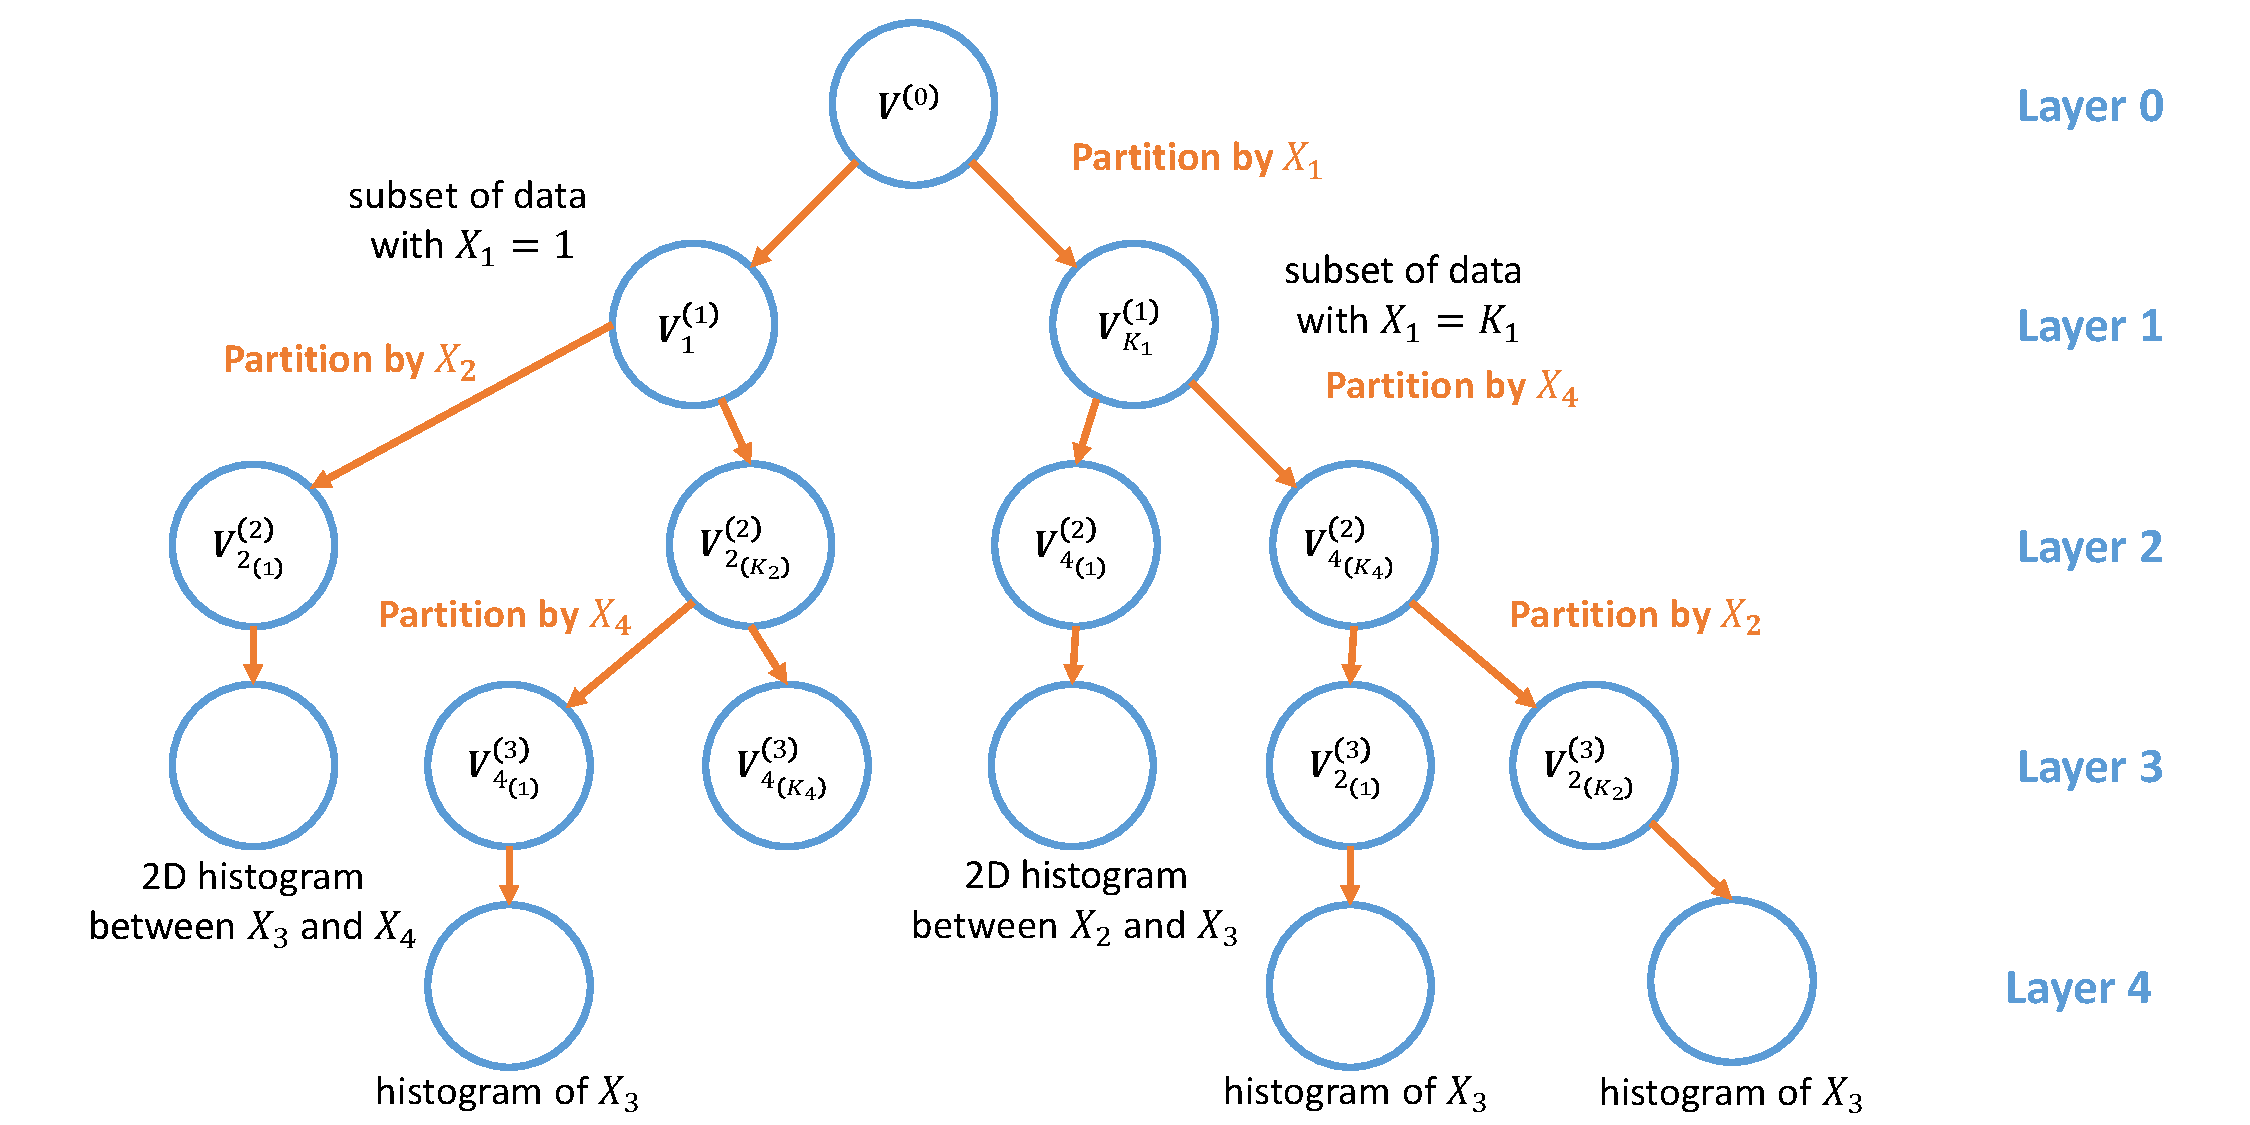
\includegraphics[width=6.5in]{STEPS.pdf}}
\caption{Illustration of an hierarchical tree built by STEPS in a 4-variable case.}\label{fig:steps}
\end{figure}
The layers are denoted by  $l=0,1,\ldots,L=4$, and the nodes in layer $l$ are denoted by $\vv^{(l)}$ and contains the subset of data following the partitioning rule till that node along the branch of the tree where the node is positioned. $\vv^{(0)}$, the node at the top of the tree $\mathcal{T}$ contains the whole data set. $K_j$ represents the number of levels of variable $X_j$. Note that the order of the variables for partitioning may differ by branch and not every branch has to be of the same length.

The sequence by which the data are partitioned or by which the attributes are aligned and placed on trees can be decided in at least two ways. First, one can leverage prior information or domain knowledge regarding the importance of the attributes, either practical or statistical, in a particular data set. This idea of applying external knowledge in developing differential privacy approaches has been used in other settings, which helps to save on privacy cost and improve the utility of released results. For example, DPFieldGroups, the method ranked fourth in the third marathon match of the 2018 National Institute of Standards and Technology Differential Privacy Synthetic Data Challenge, used external knowledge to identify highly correlated variables and grouped them before sanitization \citep{gardn999,bowen2019comparative}. The attributes that of are more of interest to practitioners would be placed more closely to the root of the tree.  

For the second approach, one may apply a metric that measures the statistical importance of an attribute based on the original data. Since this approach uses original information, it costs privacy and a portion of the total privacy budget should be allocated to keep the determination of the partitioning sequence private. For example, the metric may quantify the contribution of an attribute for explaining the variability of a count data set through loglinear models; attributes that explain more variability among a set of counts will be placed closer to the root of the tree along a branch. The metric can be a information-theoretic model selection criterion such as AIC and BIC, or other statistics for comparing the models or measuring goodness of fit of the models. If AIC is used, then the attribute used to partition the original data would be the one associated with the smallest AIC among all the univariate log-linear models fitted to the data. A similar procedure is followed during the process of growing the tree. Univariate loglinear models are applied to the subset of the data contained in a node of the tree, the attribute that is associated with the smallest AIC will be used to further partition the data contained in that node.

In the second step of sanitization and correction, differentially private noises are injected to the count in each of the nodes in the tree $\mathcal{T}$ built in the first step. To ensure the equality constraints in the hierarchical decomposition, a post-processing procedure similar to the universal histogram approach is applied, with some necessary modifications. Specifically, after the independent noise injection, the sum of the counts in the children nodes (denoted by $\mbox{succ}(v)$) are very likely not equal to the count in their parent node $v$, as they should. For example, a node $v$ contains all the  data points whose attribute ``race'' is ``white''. Say its original count of 100, and its children $\mbox{succ}(v)$ from further partitioning by ``gender''  include ``white female'' with an original count of 44  and ``white male'' of with an original count of 56. Suppose the counts are sanitized via the Laplace mechanism and become 120, 48, and 50, respectively. Then ``white male'' and ``white female'' no longer add up to ``white''.  To correct for the inconsistency in the counts between $\sum \mbox{succ}(v)$ and $v$, the inconsistent count $z$ is first calculated via Eqn (\ref{eqn:bottom}) in a bottom-up manner, and then the inconsistency is corrected to obtain the final consistent counts $\bar{n}^*$ via Eqn (\ref{eqn:top}).
\begin{equation}\label{eqn:bottom}
z[v]=
\begin{cases}
n^*[v], & \text{if } v \text{ is a leaf node}   \\
\frac{b^l-b^{L-1}}{b^L-1}n^*[v]+ \frac{b^L-b^{L-1}}{b^L-1}\sum_{u\in \mbox{succ}(v)}z[u] & \text{otherwise}
\end{cases},
\end{equation}
\begin{equation}\label{eqn:top}
\bar{n}^*[v]=
\begin{cases}
z[v], & \text{if } v \text{ is the root node}   \\
z[v]+\frac{1}{b}(\bar{n}^*[w]-\sum_{u\in succ(w)}z[u] & \text{otherwise}
\end{cases}.
\end{equation}
$b$ in Eqns (\ref{eqn:bottom}) and (\ref{eqn:top}) is the number of children per node, assumed to be the same across all nodes in $\mathcal{T}$ in the framework of the original universal histogram, and can be set by the data user ($b\ge2$). $w$ in  Eqn (\ref{eqn:top}) represents $v$'s parent. Trees generated by STEPS  might have branches of different length, but Eqns (\ref{eqn:bottom}) and (\ref{eqn:top}) would still apply. In addition, to accommodate the requirement of the same $b$ across all nodes, \emph{phantom} categories are generated so that each attribute has the same number of categories as the attribute with the most categories. The ``original'' counts in the \emph{phantom} categories are 0, and will remain at zero during the sanitization and correction process.

In the last step of synthesis and release, if all attributes are categorical, we can release directly the sanitized counts of the nodes in the bottom layer of the tree; otherwise, we can apply uniform sampling to draw synthetic values for the numerical attributes on which histograms are formed.

\subsubsection{Algorithm}
The algorithmic steps of the STEPS procedure are given in Algorithm \ref{alg:steps}. 
\begin{algorithm}[!tbh]
\caption{STatistical Election to Partition Sequentially with $L$ layers (STEPS-$L$)}\label{alg:steps}
\begin{algorithmic}[1]
\State \textbf{Input}: number of partition layers $L\; (\le p)$; overall privacy budget $\epsilon$ and the portion $r\in[0,1)$ allocated for partitioning sequence; utility function $u$ for the exponential mechanism and its sensitivity $\delta_u$; number of synthetic sets $m$; original data $D$.
\State \textbf{Output:} $m$ synthetic sets $\tilde{D}^{(1)},\ldots,\tilde{D}^{(m)}$
\State \textbf{If} there is a predefined partitioning sequence, $r=0$ and build the tree $\mathcal{T}$ according to the sequence.
\State \textbf{Else} define $\mathcal{A}^{(0)}_{v^{(0)}[1]}$ that includes all $p$ attributes in $D$.
\State \hspace{10pt} \textbf{For} $l=0$ to $L-1$
\State \hspace{20pt} \textbf{For} $k=1$ to $K^{(l)}$  ($K^{(l)}$ is number of nodes in layer $l$)
\State\hspace{26pt}$\bullet$ Apply a univariate loglinear model to the data contained in node $\vv^{(l)}[k]$ with \\ \hspace{24pt} each attribute from its availability set $\mathcal{A}^{(l)}_{\vv^{(l)}[k]}$, and obtain the model selection metric.
\State\hspace{26pt}$\bullet$ Choose a partitioning variable via the Exponential mechanism  with privacy \\ \hspace{24pt}  budget $r\epsilon/(m(L-1))$. Denote the selected attributed by $X_{j(k)}$.

\State \hspace{26 pt}$\bullet$ Exclude $X_{j(k)}$ from the availability sets for the all children nodes of $\vv^{(l)}[k]$ in \\  \hspace{30 pt} layer  $l+1$.
\State \hspace{20 pt} \textbf{End For}
\State \hspace{10 pt} Obtain the full histogram over all the attributes in $\mathcal{A}^{(L}_{\vv^{(L)}}$ for all nodes in layer $L$.
\State \hspace{10 pt} \textbf{End For}
\State \textbf{End Else}
\State  Sanitize all nodes in the generated tree $\mathcal{T}$ (e.g. via the Laplace mechanism), and apply the inconsistency correction in Eqns (\ref{eqn:bottom}) and (\ref{eqn:top}) to obtain the final sanitized counts $\bar{\mathbf{n}}^*$. 
\State  If all attributes are categorical, release the sanitized counts of the nodes in the bottom layer of $\mathcal{T}$; otherwise, apply  uniform sampling to draw synthetic values for the numerical attributes on which histograms are formed.
\end{algorithmic}
\end{algorithm}
The input to the STEPS algorithm includes a user-specified number for the partition layers $L$. If it is a full decomposition of $f(\mathbf{X})$, then $L=p$; otherwise, $L<p$. Though the case of $L>p$ is possible if we allow different levels of an attribute to span across multiple levels, this does not seem to be necessary from a data synthesis perspective, especially when the partitioning sequence is determined using the model selection approach. Therefore, we only present the case that once a variable is used in partitioning data along a branch in the tree, it is no longer available for further splitting along that branch; in other words, the set of available attributes $\mathcal{A}^{(l)}_{\vv^{(l)}[k]}$ for partitioning the $k$-th node  $\vv^{(l)}[k]$ in layer $l$ will shrink as the tree grows. When $L<p$, there  will be more than one attributes in $\mathcal{A}^{(L)}_{v^{(L)}[k]}$ for the $k$-th nodes in Layer $L$, but no more partitioning will be applied and the leaf nodes will be made of the cells from the full cross-tabulation over all the remaining attributes in $\mathcal{A}^{(L)}_{\vv^{(L)}[k]}$.

Regarding the choice of $L$ for STEPS, larger $L$ is associated with more computational complexity and less privacy budget per layer. On the other hand, it allows differentiation of more important attributes from less important ones and potentially better preservation of the original information. In addition, since the counts in top layers are weighted averages of multiple nodes per Eqn. (\ref{eqn:top}), the loss in privacy budget per layer could be offset or even trumped by the information aggregated over multiple nodes. In theory, there exists an optimal $L$  based on the trade-off between privacy budget and data utility. Users may try different values of $L$ and pick the optimal one; but the procedure of deciding on the optimal $L$, if based on the original data, itself costs privacy. For future work, we will look into devising a stopping rule for tree building rather than choosing the height of the tree beforehand. More discussions are provided in Section \ref{sec:disc}.

The overall privacy budget will split between building and sanitizing the hierarchical tree, if the data set itself is used to suggest the structure of the tree. Specifically, a certain portion $r$ of the overall privacy will be allocated to find the optimal split variable for a node via the Exponential mechanism, which is further split into $L$ partition layers.  If the structure is suggested by external knowledge, then $r=0$ and the tree building step costs no privacy. The rest of the budget $1-r$ can be used to sanitize the node counts in the constructed tree, which will also be further split into $L$ partition layers. The optimal $r$, a hyperparameter, likely depends on the data; but users could preset a $r$ value they are willing to spend on tree building if they do not want to spend budget to pick $r$. Since different nodes in the same layer do not have overlapping information, choosing the split variables and sanitation of the nodes follow the parallel composition principle. Taken together, with $m$ synthetic data sets, and if each layer receives the same amount of budget for count sanitization, then each node count in layer $l$ receives a budget of $(1-r)\epsilon/(mL)$.

If there is pre-defined partitioning sequence, the exponential mechanism is used to privately choose a partitioning variable for each node $v$  out of all attributes $\in\mathcal{A}_v$ until layer $L$. Specifically, it samples attribute  $j\in\mathcal{A}_v$ with probability 
\begin{equation}\label{eqn:exp}
\textstyle = \exp(u_j(v)) \frac{\epsilon}{2\delta_u} )/\sum_{k\in\mathcal{A}_v} \exp\left(u_k(v) \frac{\epsilon}{2\delta_u}\right),    
\end{equation} 
where $\delta_u$ is the maximum change in the utility function $u$ with one element change in the data contained in $v$. A reasonable choice for $u$ is AIC, whose  $\delta_u=2$ per Lemma  \ref{lem:AIC}.
\begin{lem}[Sensitivity of AIC in univariate loglinear model]\label{lem:AIC} Let the utility function $u$ in the Exponential mechanism be the AIC in the univariate log-linear model with a single attribute. $\delta_u$  is equal to 2. 
\end{lem}
\begin{proof}
AIC $=-2\log(\mathcal{L}) + 2K$, where $\mathcal{L}$ is the likelihood function and $K$ is the number of the parameter of the model. For the univariate log-linear model with an independent variable of $K$ levels, $\mathcal{L}=\frac{n_v!}{\prod_{k=1}^K n_{v,k}! } \prod_{k=1}^Kp_k^{n_{v,k}}$ and $\log(\mathcal{L})=\log(n_v!)-\sum_{k=1}^K \log(n_{v,k}!)+\sum_{k=1}^K n_{v,k}\log(p_k)$, where $n_v$ is the data size, and $n_{k,v}$ is the count in level $k$ of that attribute.  Removing one element from $v$ leads to a loss of one observation in one of the $K$ categories, say level $j$. The likelihood function based on the $n_v-1$ observation is 
$L'=\frac{(n_v-1)!}{(n_{v,j}-1)!\prod_{k\ne j} n_{v,k}!} p_j^{n_{v,j}-1} \prod_{k\ne j} p_k^{n_{v,k}} $ and  $\log(\mathcal{L}')=\log((n_v-1)!)-\log((n_{v,j}-1)!)-\sum_{k\ne j} \log(n_{v,k}!)+n_k\log(p_k)+\sum_{k=1}^K n_{v,k}\log(p_k)$.  Therefore, the change in AIC is $\Delta$AIC$=-2\log(\mathcal{L})+2K+2\log(\mathcal{L}')-2K'$ with the removal of one attribute. Plugging the log-likelihoods, we have $\Delta$AIC$=\log(n_v)-\log(n_{v,j})+n_{n,j}\log(p_j)-(n_{n,j}-1)\log(p_j) +2K-2K'$. The true parameter $p_j$ is unknown and its maximum likelihood estimate is $n_{v,j}/n_v$ and  $(n_{v,j}-1)/(n_v-1)$ before and after removing an observation. Therefore, $\Delta$AIC 
$=\log(n_v)-\log(n_{v,j})+n_{v,j}\log(n_{v,j}/n_v)-(n_{n,j}-1)\log((n_{v,j}-1)/(n_v-1)) +2K-2K'= (n_{v,j}-1)\log(n_{v,j}(n_v-1)/(n_v(n_{v,j}-1))+2K-2K'$. When $n_j\ge2$, $K=K'$ and thus $\Delta$AIC 
$=(n_{v,j}-1)\log(n_{v,j}(n_v-1)/(n_v(n_{v,j}-1)) \in(0,1)$. When $n_j=1$, then $K'=K-1$, and $\Delta$AIC$=2$. Taken together, $\delta_u$ with AIC is 2
\end{proof}

Plugging $\delta_u =2 $ in Eqn (\ref{eqn:exp}), then attribute $j$ is sampled with probability
\begin{align}
&\textstyle= \exp(-\mbox{AIC}_j\epsilon/4)/\sum_k\exp\left(-\mbox{AIC}_j\epsilon/4\right)\notag\\
&\textstyle= \exp\left([\max_{j'}\mbox{AIC}_{j'}-\mbox{AIC}_j)] \epsilon/4\right)/\sum_k\exp\left([\max_{j'}\mbox{AIC}_{j'}-\mbox{AIC}_j]\epsilon/4\right)\label{eqn:AIC2}
\end{align}
Eqn.  (\ref{eqn:AIC2}) is likely to be more practical from a computational perspective so to reduce numerical errors. 

\begin{rem}[Generalization of  Algorithm \ref{alg:steps}]\label{rem:alg}
The algorithm presented in Algorithm \ref{alg:steps} may have other variants. For example, rather than using AIC as the utility function for the Exponential mechanism, we could use a metric to measure the dissimilarity among different clustering of the attributes in terms of their importance, and STEPS will partition the data by a group of variables per layer rather than by a single attribute per layer. For example, suppose there are 5 variables and $L$ is pre-set at 2. After obtaining their respective AIC values, the Exponential mechanism is applied to choose among 15 different ways of grouping of the variables into two clusters (5 ways of 1:4 partitioning between Layer 1 and 2, 5 ways of 4:1 partitioning between Layer 1 and 2), and the the grouping scheme with the largest average difference between will used, and the group with the smaller average AIC in that scheme is placed in Layer 1. This generalized scheme is what is used in the simulation studies.
\end{rem}

\subsection{Difference between STEPS and other partitioning approaches}\label{sec:UH}

The STEPS procedure focuses on constructing a differentially private joint distribution, in relatively high dimensional settings, from which synthetic data are generated. It aims at  better  preserving information for important variables, where ``important'' can be defined either statistically or per domain knowledge. To the best of our knowledge, STEPS seems to be only approach that explores the potentials of the decomposition sequence of the joint distribution of the attributes to improve the utility of synthetic data. By contrast, most existing partitioning approaches focus on improving the accuracy of marginal counts in low-dimensional setting. In addition, they often allow the same attribute to span multiple layers whereas different layers in STEPS contains non-overlapping attributes. 

Among the existing partitioning-based DP approaches, STEPS perhaps relate to the universal histogram the most as it uses the inconsistency correction rules developed in the latter. Exploring and maintaining the inherent consistency constraints is the main reasons why the universal histogram procedure improves the accuracy of low-dimensional marginal queries. The universal histogram is mostly studied in the context of a single attribute, where the high-level nodes present large-range queries and the leaf nodes in the lowest level are the finest categories/bins for the attribute. Though it can be applied to multidimensional data, its benefit over the one-step Laplace sanitizer seems to diminish over increasing dimensionality \citep{qardaji2013understanding,qardaji2013geo}. In addition, the universal histogram approach has an exponential time complexity $O(b^L)$ in $L$ for a given $b$ (Eqns (\ref{eqn:bottom}) and (\ref{eqn:top})), implying a large $L$ would dramatically increase the computational time \citep{qardaji2013understanding}.

%%%%%%%%%%%%%%%%%%%%%%%%%%%%%%%%%%%%%%%%%%%%%%%%%%%%%%%%%%%%%%%%%%%%
% Simulation
%%%%%%%%%%%%%%%%%%%%%%%%%%%%%%%%%%%%%%%%%%%%%%%%%%%%%%%%%%%%%%%%%%%%
\section{Simulation Studies}\label{sec:simulation}
In this section, we implement the STEPS method in simulated data to generate differentially private synthetic data, and compare the utility of the synthesized data with those generated via a modified version of the universal histogram, and PrivBayes. %, and the flat Laplace sanitizer. 

\subsection{Choice of methods for comparison}
The reasons for choosing the two methods (universal histogram and PrivBayes) to compare with STEPS are detailed below. 

As mentioned above, STEPS uses the inconsistency correction rules developed in the universal histogram during its second step of sanitization and correction. Thus, it makes sense to include the universal histogram in the comparison set. However, we will make some modification to the original universal histogram to accommodate the computational constraints and to handle multi-dimensional data ($p=5$ in the simulation and $p=15$ in the case study in Sec \ref{sec:voter}). In addition, \citet{qardaji2013understanding} suggest that the universal histogram  generally is the best data-independent algorithm and achieves lower error for range queries from 1D histogram, compared to many data-independent methods such as the flat Laplace sanitizer and Privelet. 

STEPS has a similar framework as PrivBayes \citep{zhang2017privbayes}. Both methods build a differentially private joint distribution among the data attributes first from which synthetic data are generated. For PrivBayes, the joint distribution is obtained from the Bayesian network, which explores conditional independence among the attributes. This is different from STEPS, which still builds a full-dimensional empirical distribution but allocates different amount of privacy budgets to different attributes in the data according to their importance level. Similar to STEPS, PrivBayes can also deal with numerical attributes with discretizing into histogram bins. 

While there are other DP methods out there that can be potentially used for data synthesis, such as the 10+ competing methods for answering range queries from 1D and 2D histograms examined in \citet{hay2016principled}, we do not examine most of these methods in our empirical studies (simulation studies in this section as well as the case study in Sec \ref{sec:voter}), as explained below. The DAWA method \citep{dawa} performs the best overall and beat other methods such as DPcube \citep{DPcube}, MWEM \citep{hardt2012simple}, and Privelet \citep{privelet} according to \citet{hay2016principled}. However, we do not include DAWA due to a couple of reasons. First, it is developed for answering range queries in low-dimensional histograms (the original paper focuses on 1D histogram only) our data have a much large $p$. Second, another major reason that DAWA outperforms other methods for releasing histograms is that it allocates a certain privacy budget to identify an optimal bucketing scheme on the numerical attribute before injecting noise. Given most of the attributes our simulated and case study are either categorical or ordinal with limited number of levels, the advantages of DAWA will not be brought into full play. Other methods not included for comparison include Privelet, DPcube, MODIPS, DPcopula, and MWEM due to the following reasons. Privelet and DPcube do not offer better performance than the universal histogram approach in general even in the low-dimensional setting according to the study in \citet{hay2016principled}. Since we will compare to the universal histogram, it is not necessary to have Privelet and DPcube. The MODIPS method is model-dependent and sanitizes the sufficient statistics associated with a selected model. There are a couple of downsides for MODIPS. First, not every sufficient statistic to easy to sanitize; second, a mis-specified model would generate biased synthetic data. DPcopula uses copula to model the pairwise dependency among the attributes. Not only copula assumes continuous marginal CDFs, which our simulation and case study has almost all attributes as categorical or ordinal, the synthetic data can also be sensitive to the type of copula employed. The main goal of MWEM is to obtain differentially private queries rather than generating synthetic data from an empirical distribution. To use MWEM for data synthesis, choosing a good set of queries that represents the information of the original data is vital for the quality of the synthetic data. Even with a good set of queries to start with, it does not outperform the flat Laplace sanitizer when generating synthetic data \citep{cipher}. In addition, MWEM is proved to be inconsistent and its performance highly depends on the number of iterations \citep{hay2016principled, dawa, cipher}.  

\subsection{Simulation settings}
We simulated the data from two linear regression models. Model 1 is $Y=\beta_0+\sum_{j=1}^{10}\beta_jX_j+\epsilon$, where $\epsilon\sim N(0,1)$, $X_1$ to $X_4$ are categorical predictors with 2, 3, 4 and 5 levels respectively, the true parameter values are $0,0.5,(0.5,-0.8),(1,0.5,0.5),(0.5,0.7,0.8,0.5)$, respectively. Model 1 is a main-effect model. Model 2 $Y=\bs\beta^T \mathbf{X}_{1234}+\epsilon$ is a saturated model, where $\epsilon\sim N(0,1)$, $ \mathbf{X}_{1234}$ refers the 4-way interaction term among $X_1, X_2,X_3,X_4$, and $\bs\beta$ is of dimension 120 and is sampled from a standard normal distribution. The two models represent the two extremes of a wide spectrum of possible models with 4 predictors.

For each model, we simulated 200 data sets. We also examined two sample sizes scenarios: $n=10,000$ and $n=4,000$. For the privacy budget $\epsilon$, we used $0.5, 2, 5, 10$. For each of the 12 simulation scenarios (2 models at 2 sample sizes with 3 $\epsilon$), four sets of synthetic data were generated  by each of the three DIPS approaches. Since each approach works on categorical data, each method works on the histogram formed from $Y$ (15 bins) rather than on $Y$ directly. Once the count data were sanitized, numerical values for $Y$ can be sampled uniformly in each non-empty bin.

For STEPS, we set $L=2$ and split the total $\epsilon$ in $1:9$ ratio for building the tree via the Exponential mechanism vs sanitizing the counts via the Laplace mechanism. As mentioned in Remark \ref{rem:alg}, the generalized algorithm was applied and in most cases, the group of $(X_1,X_2,X_4)$ has much smaller AIC than the group of $(X_3,Y)$ and ends up as the partitioning variables in the first layer. We modified the original universal histogram to allow unequal number of children per node and to handle categorical attributes. In other words, the modified universal histogram is more of a STEPS procedure with a random partitioning sequence. We set $L=4$ in the modified universal histogram. For PrivBayes, we applied the Python codes by \citet{ DataSynthesizerpaper}, available at GitHub \citep{DataSynthesizercodes}. For all simulation scenario settings, the degree of the Bayes network was set at 2. The total $\epsilon$ was split in half between choosing a Bayesian network vs. sanitizing the joint distribution among the attributes based on the chosen Bayesian network.

We run the true underlying linear regression model on each synthetic set and the inferences on the regression coefficients were summarized via the combination rule listed in \citet{liu2016model} and \citet{bowen2016differentially}. For the saturated model case, the ridge regression is used due to the large number of parameters and likelihood of linear dependent matrix $\mathbf{X}^T\mathbf{X}$. The bias, root mean squared error (RMSE), and coverage probability (CP) of the 95\% confidence interval (CI) are summarized for each regression coefficient in each model. In addition, the estimated private models were used to predict the outcome in an independent testing data set of $n=100$, and the prediction MSE were obtained.

\subsection{Results}
The results are presented in Figures \ref{fig:maineffect} and \ref{fig:saturated} for the main-effect model and the saturated model, respectively. 

When the true model contains only the main effects, PrivBayes performs the best in terms of parameter estimation bias, CP, and the prediction RMSE; and STEPS performs the best in terms of parameter estimation RMSE. PrivBayes is the worst in parameter estimation RMSE, and the modified universal histogram (UH) or UH modified is the worst in parameter estimation bias, CP, and the prediction RMSE. As expected, the inferences improve as $n$ or $\epsilon$ increases with the only exception in the case of CP across $\epsilon$ for PrivBayes at both $n$ scenarios. Specifically, the trend in CP for PrivBayes are rather counter intuitive: the larger $\epsilon$ is, the more deviation there is from the nominal 95\% level. This is likely due to the discretization in $Y$. When $\epsilon$ is large, the synthetic data look similar to the original empirical distribution, but with the (deterministically) discretized $Y$, and the main source of information loss is due to the discretization in $Y$ rather than due to the sanitization. The main source of variation across the multiple synthetic sets is due to the sampling in each bin of $Y$, which is not meant to comprehend the information loss due to the discretization. On the contrary, at small $\epsilon$, the main source of information loss is due to sanitization, and releasing multiple synthetic sets is designed to take into account and the inferences are rather better than those at large $\epsilon$.

When the true model is saturated, STEPS performs the best in terms of parameter estimation bias, CP, RMSE, and the prediction RMSE; and PrivBayes is the worst in parameter estimation RMSE, and the UH modified is the worst in the CP and the prediction RMSE. For STEPS, the inferences improve as $n$ or $\epsilon$ increases, as expected, with the only exception in the case of CP across $\epsilon$ at both $n$ scenarios, which is likely due to the same reason as discussed above in the case PrivBayes in the main-effect model. For the UH modified, the inferences get better as $n$ increases, but the trend is not obvious across $\epsilon$. For PrivBayes, the trends across $n$ and $\epsilon$ are not obvious in any of the four examined metrics.  
\begin{figure}[!htb]
\small{para. est. bias$\;\quad$}
\raisebox{-0.5\height}{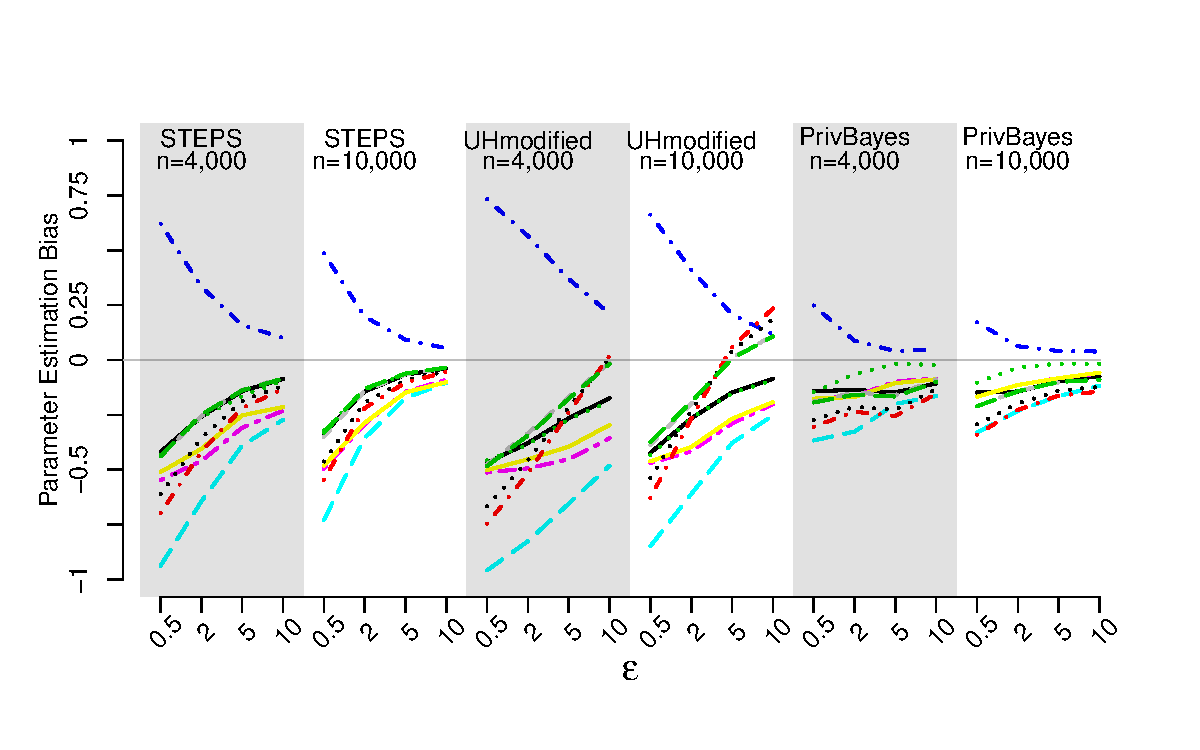
\includegraphics[scale=0.552]{bias.pdf}}\\
\small{para. est. RMSE}
\raisebox{-0.5\height}{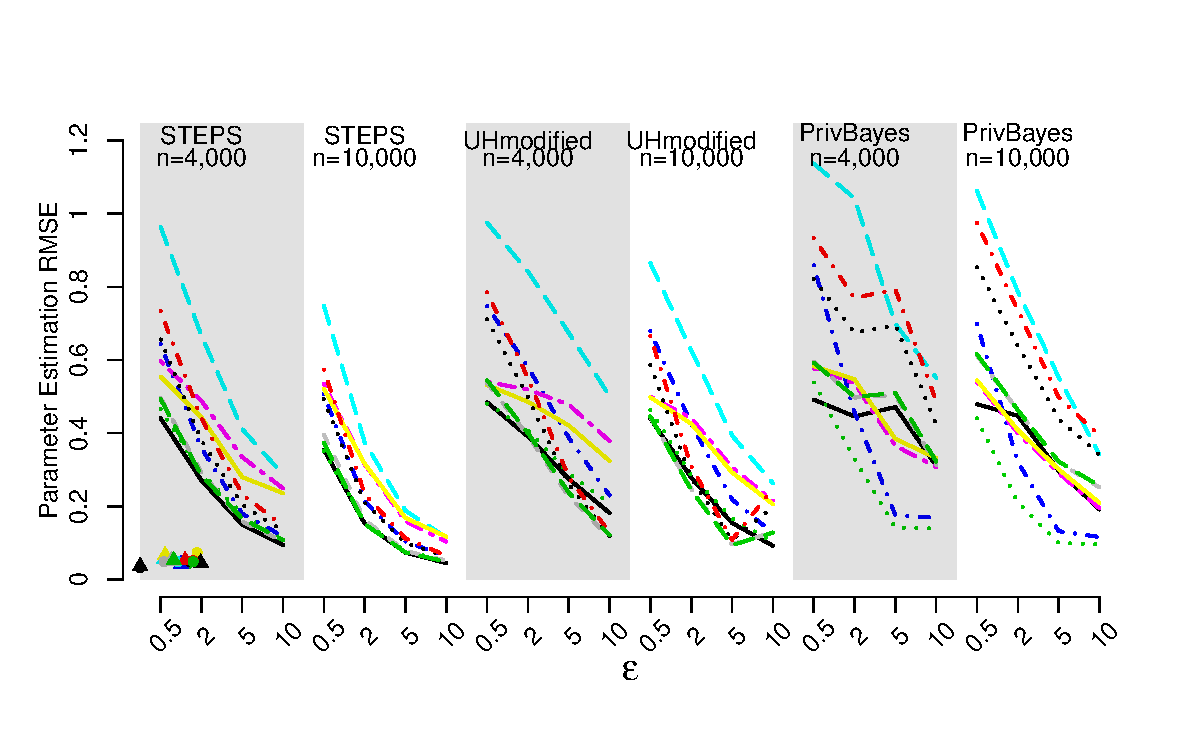
\includegraphics[scale=0.552]{RMSE.pdf}}\\
\small{CP of 95\% CI$\;\quad$}
\raisebox{-0.5\height}{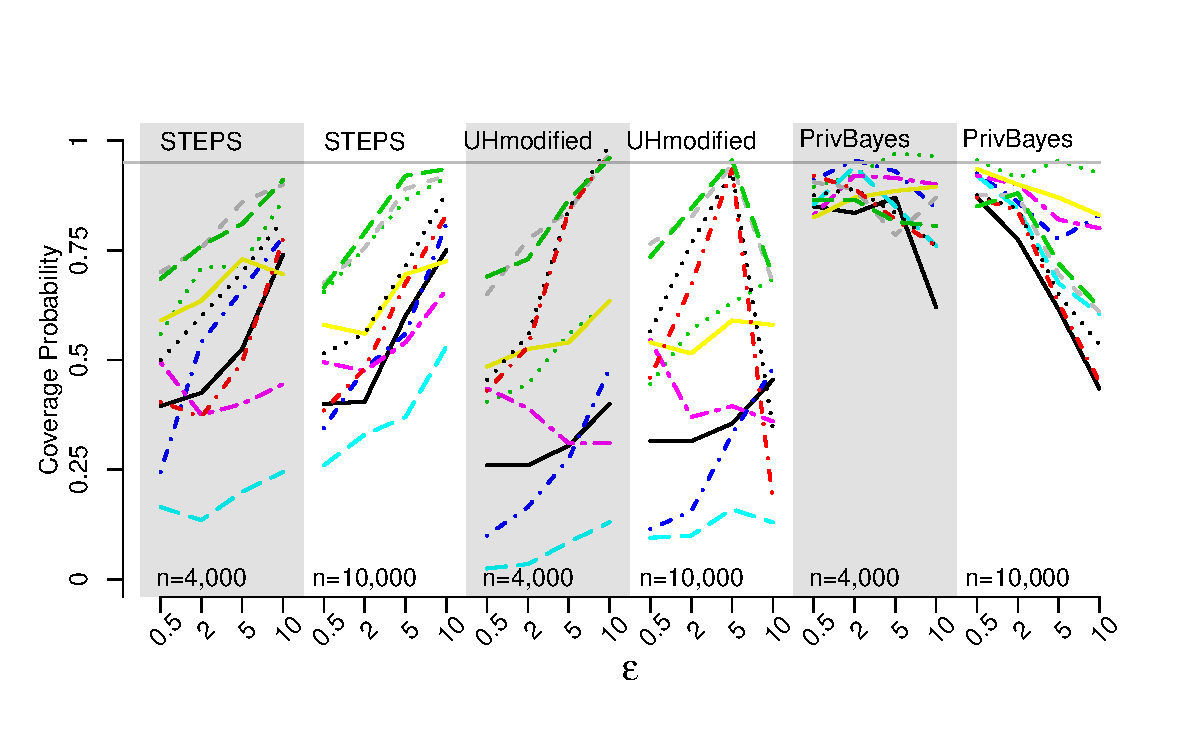
\includegraphics[scale=0.552]{CP.pdf}}\\
\small{prediction RMSE}
\raisebox{-0.5\height}{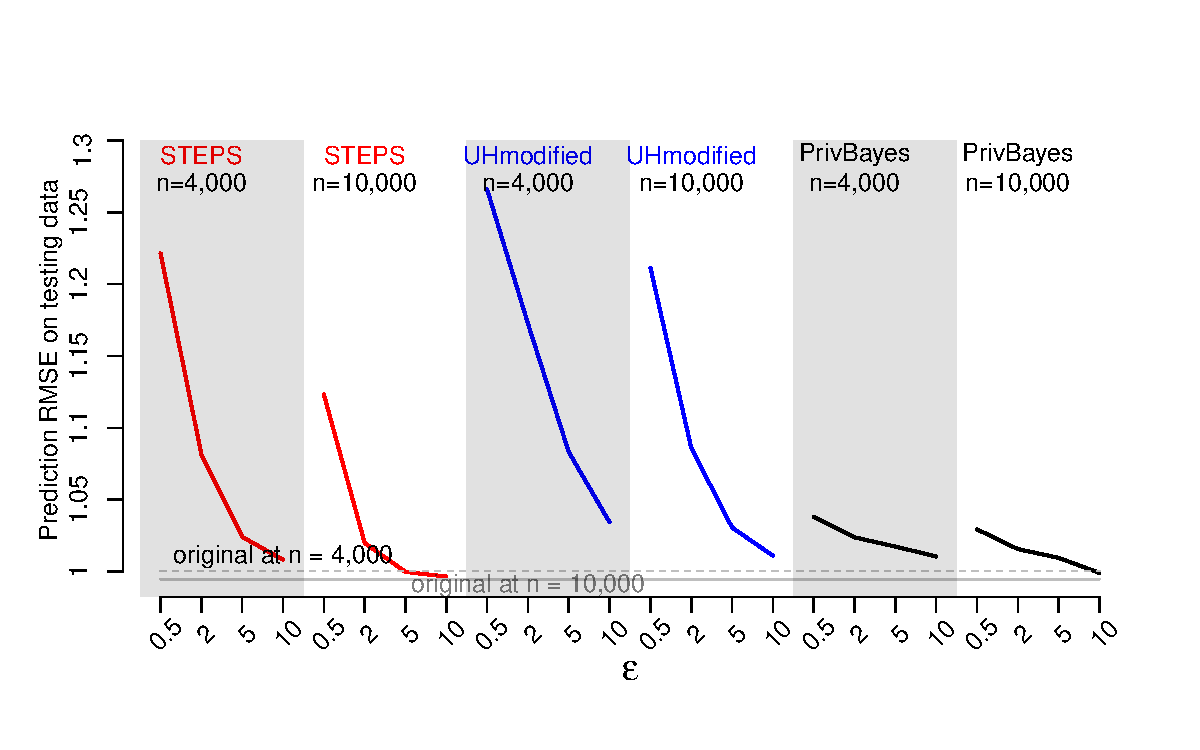
\includegraphics[scale=0.552]{RMSEtest.pdf}}\vspace{-9pt}
\caption{Inferences based on differentially private synthetic Data in the simulation study. In the top 3 plots, each line presents a different regression coefficient in the main-effect linear model}\label{fig:maineffect}\vspace{-12pt}
\end{figure}

\begin{figure}[!htb]
\small{para. est. bias$\;\quad$}
\raisebox{-0.5\height}{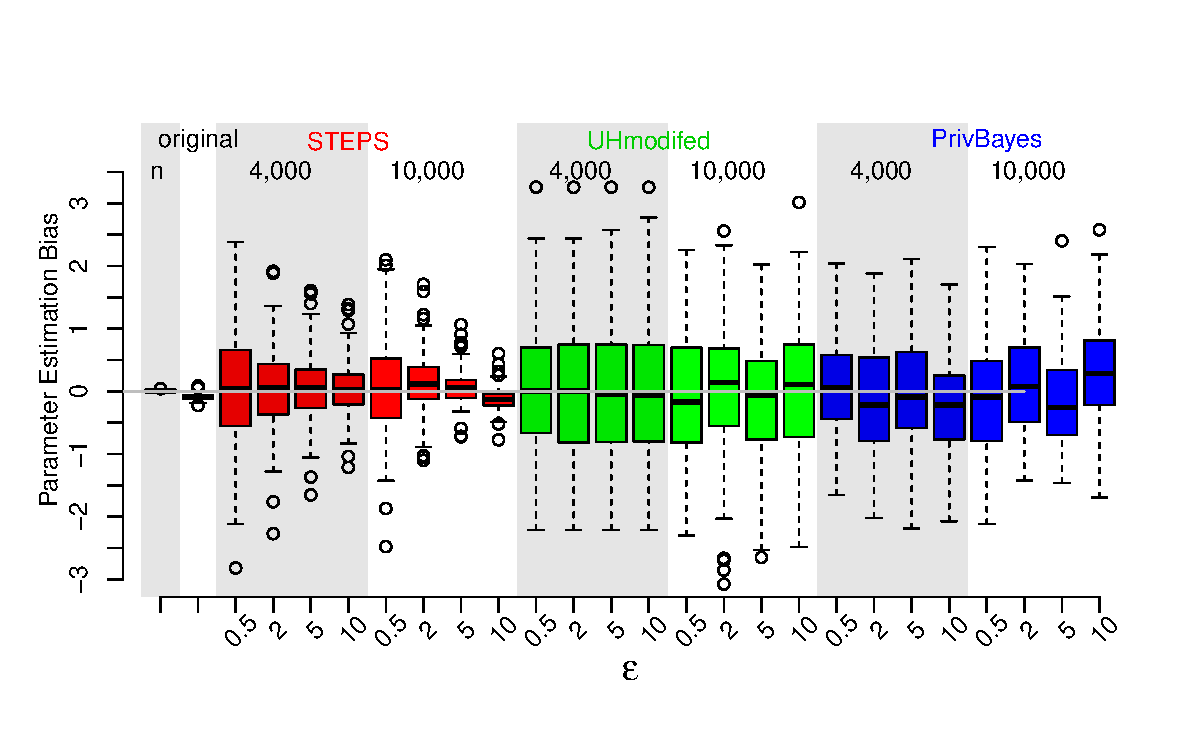
\includegraphics[scale=0.551]{biasS.pdf}}\\
\small{para. est. RMSE}
\raisebox{-0.5\height}{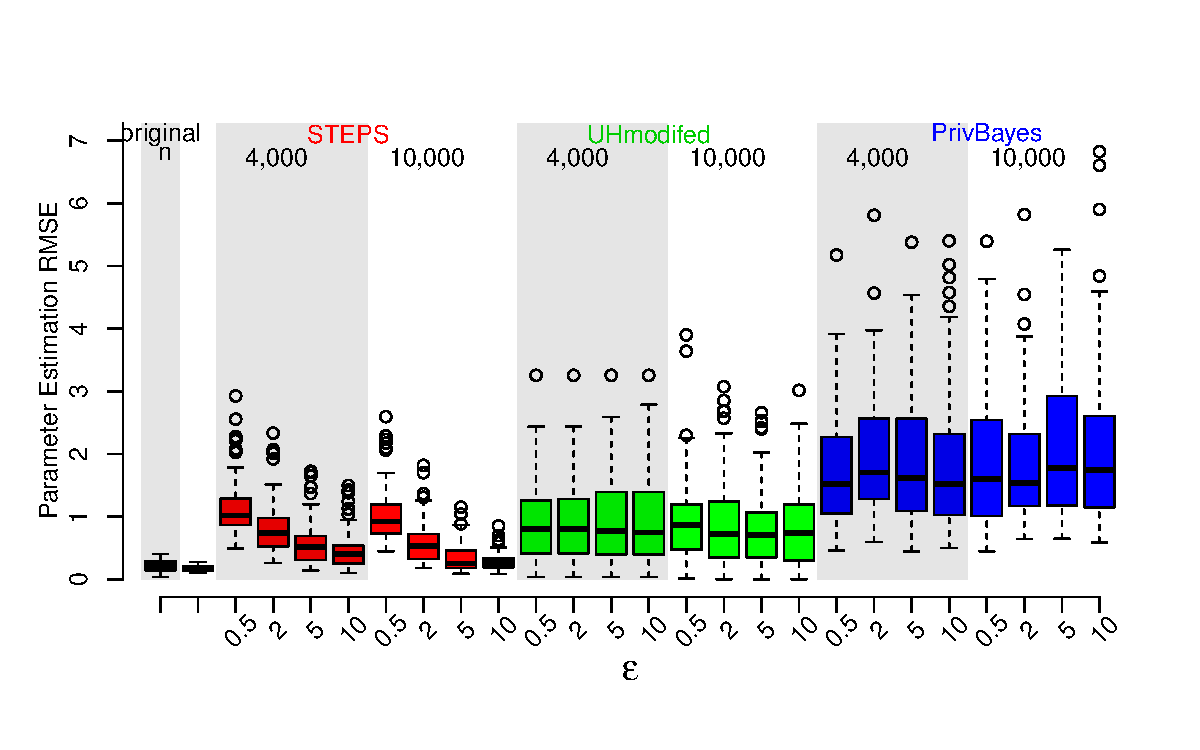
\includegraphics[scale=0.551]{RMSES.pdf}}\\
\small{CP of 95\% CI$\;\quad$}
\raisebox{-0.5\height}{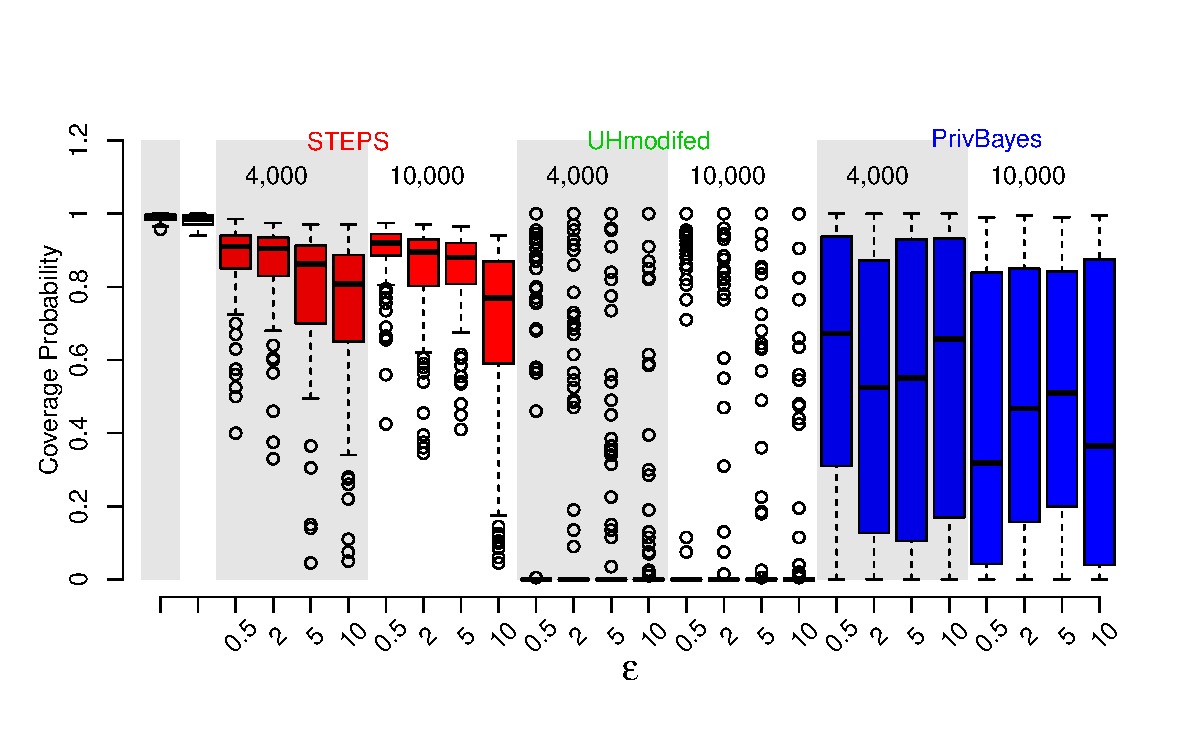
\includegraphics[scale=0.551]{CPS.pdf}}\\
\small{prediction RMSE}
\raisebox{-0.5\height}{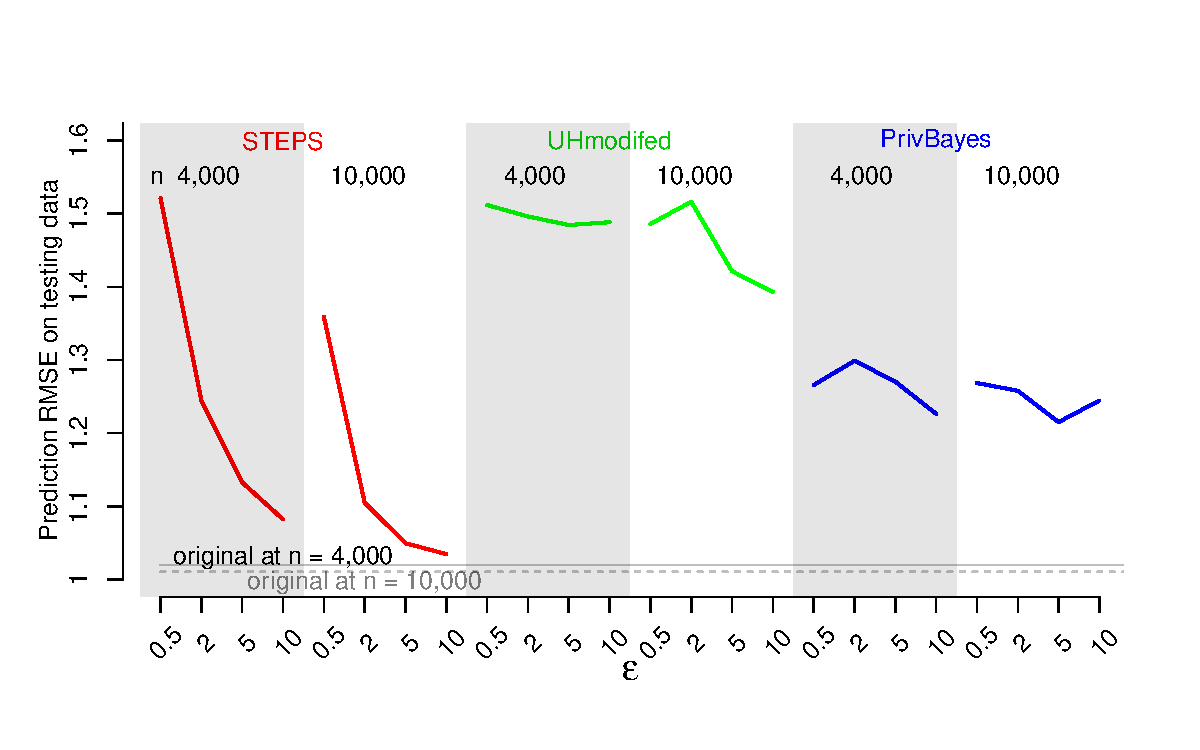
\includegraphics[scale=0.551]{RMSEtestS.pdf}}\vspace{-9pt}
\caption{Inferences based on differentially private synthetic Data  in the simulation study. In the top 3 plots, each line presents a different regression coefficient in the saturated linear model.}\label{fig:saturated}\vspace{-12pt}
\end{figure}

%%%%%%%%%%%%%%%%%%%%%%%%%%%%%%%%%%%%%%%%%%%%%%%%%%%%%%%%%%%%%%%%%%%%
% Case Study
%%%%%%%%%%%%%%%%%%%%%%%%%%%%%%%%%%%%%%%%%%%%%%%%%%%%%%%%%%%%%%%%%%%%
\section{Application to the 2002-2012 CPS Youth Voter Data}\label{sec:voter}

\subsection{Data Description}
The 2000-2012 Current Population Survey (CPS) is downloaded from the Harvard Dataverse \citep{Dataverse}. The CPS is the primary source of labor force statistics for the population of the United States. In election years, the CPS also collects data on reported voting and registration, provides a large and nationally representative sample with coverage of both registered and non-registered individuals, reports statistics on the voter turnout, age, race, among others. The voting and registration data from CPS are frequently used and cited by various news outlets such as Time \citep{Time}, New York Times \citep{NYT}, Fortune \citep{Fortune}, and Newswise \citep{Newwise}, among others. 

In this application, we focus on the youth voter subset. The data was used to examine the effect of preregistration laws on turnout among young voters \citep{Holbein2016}. The data set has $n=44,821$ observations and $p=15$ variables  (Table \ref{tab:datlist}), and contains sensitive attributes such as Family Income and Voted. The data also contains pseudo-identifiers such as gender, race information, and location information, which can be used by data intruders to identify subjects or to link to other databases. Therefore, it is important to make sure individual information is protected before the data set, or its synthetic copies, are released. 
\begin{table}[!htb]
\centering
\resizebox{0.9\textwidth}{!}{
\begin{tabular}{@{}L{2.1in}@{}| L{4.1in}@{} }
\hline
Variable & category (percentage)\\
\hline
Voted &yes (34.7), no (63.3) \\
Preregistration State & yes (10.5), no (89.5)\\
Age (years) & 18 (20.5), 19 (19.7), 20 (20.0), 21 (20.0), 22 (19.8)\\
Married &  yes (7.5), no (92.5)\\
Female & yes (50.7), no (40.3)\\
Family Income$^\ddag$ & 14 levels (3.1, 5.9, 26.5)$^\ddag$ \\
College Degree & yes (3.1), no (96.9)\\
White &yes (69.3), no (31.7)\\
Hispanic &yes (14.6), no (85.4)\\
Registration Status & yes (52.4),  yes (47.8)\\
Metropolitan Area &yes (77.9), no (22.1)\\
Length of Residence & $<$1 month (2.7),
1-6 months (20.0),
7-11 months (6.9),
1-2 years (15.0),
3-4 years (9.8),
$\ge5$ years (45.6)\\
Business/Farm Employment & yes (12.6), no (12.62)\\
In-Person Interview &yes (36.7), no (63.3)\\
DMV Registration &yes (12.7), no (87.3)\\
\hline
\end{tabular}}
\resizebox{0.9\textwidth}{!}{\begin{tabular}{l}
\footnotesize For Family Income, the minimum, maximum and medium percentage among the 14 levels are listed.\\
\hline
\end{tabular}}
\caption{List of variables and their values from youth voter subset in the 2000-2012 CPS data.}
\label{tab:datlist}
\end{table}

%---------------------------
\subsection{Implementation}\label{sec:stepsinvoter}
Similar the simulation studies, we compare the STEPS procedure in data utility against the modified universal histogram approach, and the PrivBayes. In addition, we include the flat Laplace sanitizer as another benchmark. \citep{hay2016principled} concluded when $n$ or privacy budget is large, it is unlikely that any of the more complex algorithms will beat a simpler and easier-to-deploy flat algorithm. Similar observations regarding the Laplace sanitizer are also obtained in the empirical studies conducted in \citet{bowen2016differentially}, especially when $p$ is large. The voter data has a large $n$ ($44,821$) and relatively large $p$ (15), which will be a good case study on how the flat Laplace sanitizer performs considering its simplicity for practical implementation.

Table \ref{tab:datlist} shows most attributes in the youth voter data set are categorical and with ``age'' being the only continuous variable. Since this numerical attribute take on limited number of values (ages 18 to 22) and to avoid discretizing the numerical attributes in an ad-hoc manner during the application of the DIPS methods, we treat all attributes as categorical.

For STEPS, we applied Algorithm \ref{alg:steps} and selected the optimal variable for node splitting by leveraging domain knowledge. We used expert knowledge instead of using the Exponential mechanism to demonstrate how the data curator could save all the privacy budget for the sanitization step. 

Our domain expert, a public policy researcher at the Urban Institute, suggested  that ``Voted'', ``College Degree'', and ``Preregistration State'' are the top three important variables to practitioners in this data set. ``Voted'' is ranked first, because this is voter data set and ``voted'' is perhaps the variable that is of interest to most researchers and practitioners who use data. Also, the attribute presents an important predictor for turnout in future elections. In the Ohio 2000 election, if a voter voted in one of the past four general or primary elections, they had a 70\% probably of voting whereas if they voted in two of those elections, they had a 90\% probability of voting \citep{malchow2004predicting}. ``College Degree'' is ranked the second since scholars have consistently noted that highly educated individuals participate in politics more than the average citizen \citep{campbell1980american, rosenstone1993mobilization}. Some researchers have also concluded that education is the socio-demographic variable most strongly correlated with turnout \citep{wolfinger1980votes}, which also relates to education status. The third variable is ``Pre-registration State''. \citet{mcdonald2010registering} found higher turnout rates in Florida and Hawaii among those who preregistered (registered before they were able to take part in the next election) compared to those who registered after they turned 18. Pre-registrants were 4.7\% more likely to vote in the 2008 election than those who registered after they turned 18. For comparison, we built a tree with two partitioning layers $L=2$ (partitioning by ``voted'' then ``College Degree''), and a tree with three partitioning layers $L=3$ (partitioning by ``voted'' then ``College Degree'', then ``Pre-registration State''). Figure \ref{fig:tree} shows what the tree structure for STEPS when $L=2$. Here ``family income'' has the most categories, that is, $b=14$, thus \emph{phantom} categories are created to make each attribute have 14 categories.

\begin{figure}[!htb]
\centerline{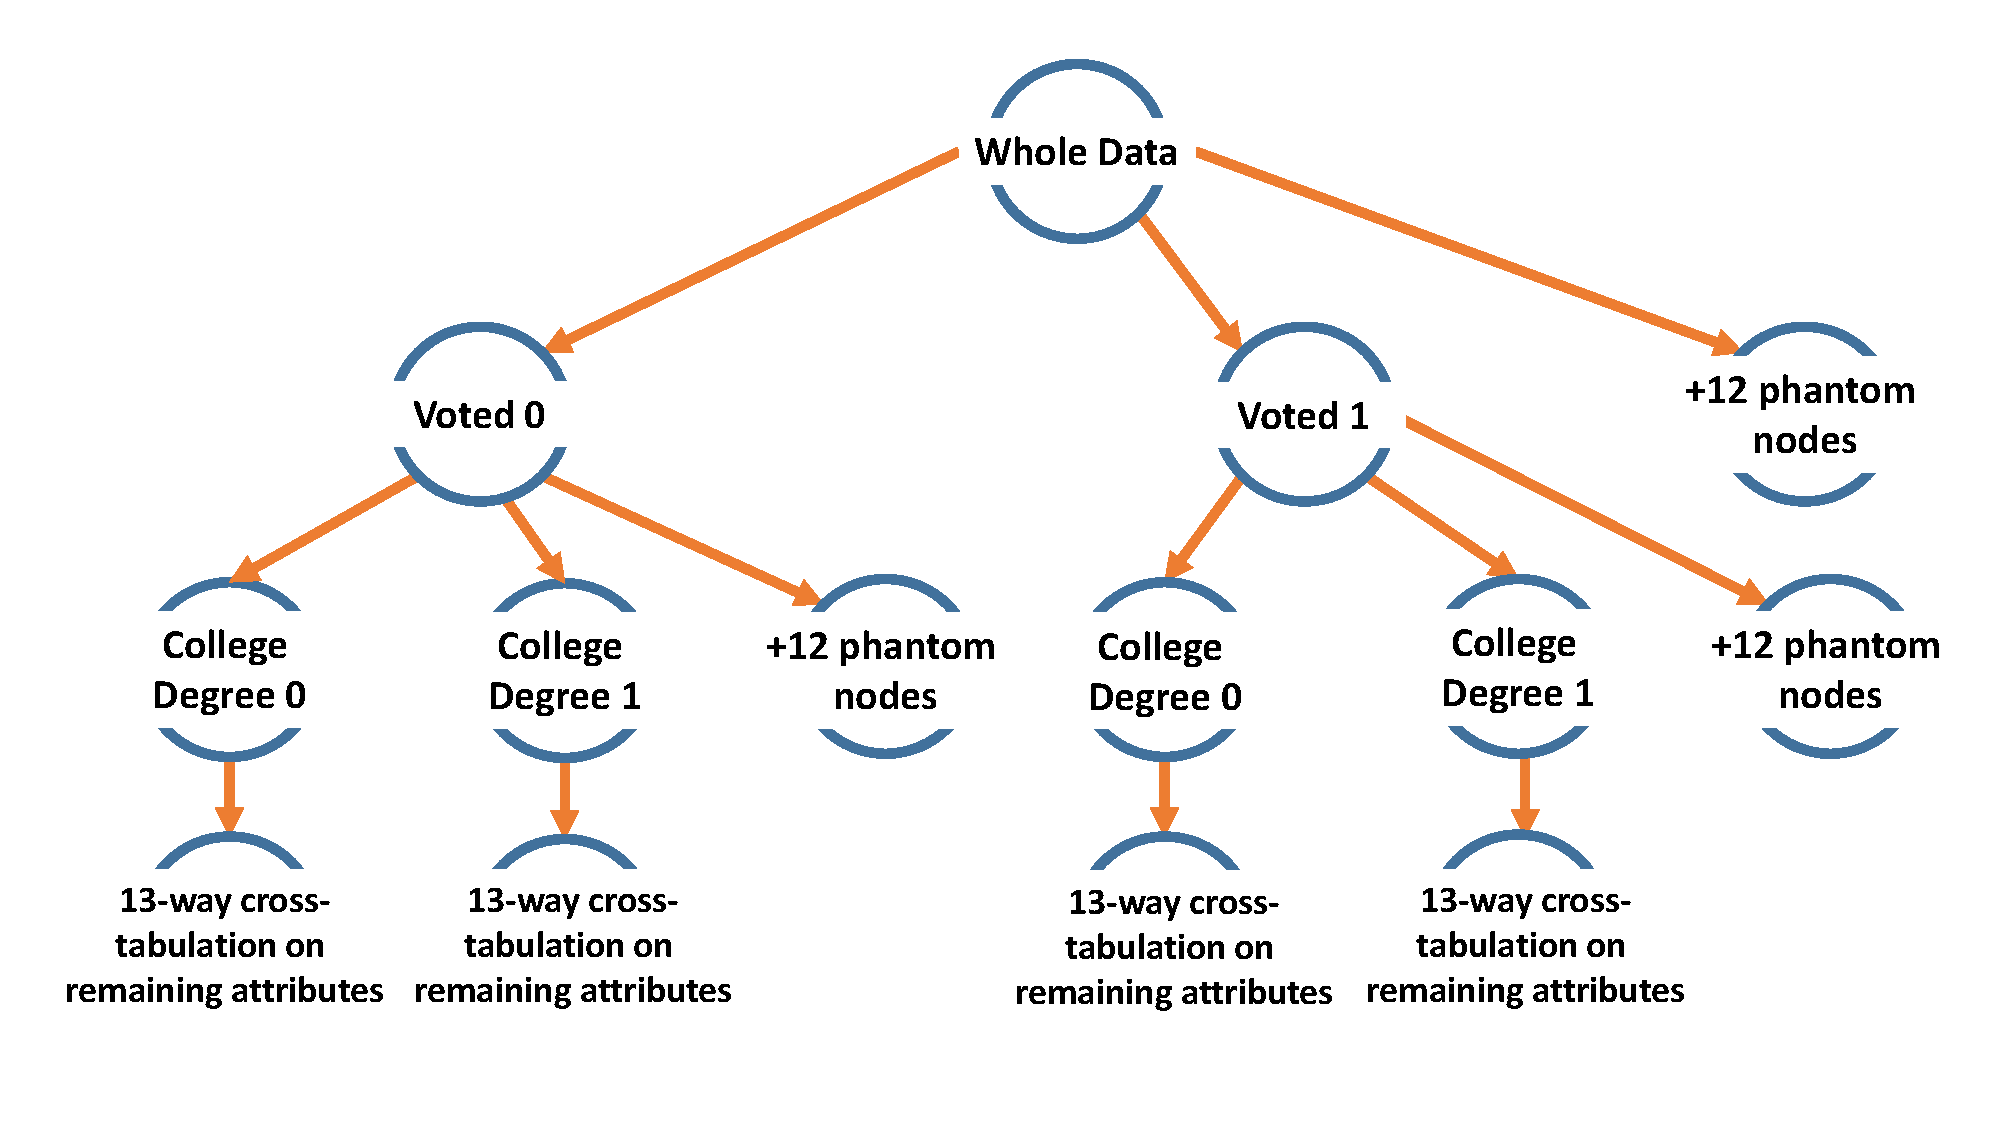
\includegraphics[width=6in]{STEPS-figure.pdf}}\vspace{-6pt}
\caption{A sketch of the constructed tree in STEPS-2.}\label{fig:tree}
\end{figure}
These phantom categories  are created solely for the purposes of applying the universal histogram procedure and always have zero counts; and they will be removed once the synthetic data are generated. 

The flat Laplace sanitizer is simple and straightforward to apply. It injects noise from Lap$(0, \epsilon^{-1})$ to each of the $1,290,240$ cells, after removing the impossible case of a person voting if they are not registered, from the  15-way cross-tabulation (Table \ref{tab:cell}). Given the enormous number of cells and a limited number of observations, the majority of the cells are empty (98.35\%). Given that the empty cells are sample zeros rather than population zeros, they should and were sanitized.

\begin{table}[!htb]\centering
\resizebox{0.8\textwidth}{!}{
\begin{tabular}{ c | c c c c c c c}
\hline
Cell size & 0 & 1 & 2 &3 & 4 & 5 & $\boldsymbol{>}$ 5\\
\hline
Number of Cells & 1,268,911 & 14,061 & 3,545 & 1,508 & 740 & 425 & 1,050 \\
\hline
Proportion & 98.35\% & 1.09\% & 0.27\% & 0.12\% & 0.06\% & 0.03\% & 0.08\% \\
\hline
\end{tabular}}
\caption{Summary of cell sizes and frequencies in the full cross tabulation of the youth voter data.}\label{tab:cell}
\end{table}

We did not set the number of layers in the modified universal histogram at $L=\log_bN$ per the original paper's suggestion \cite{hay2010boosting}, but used $L=2$ and $L=3$. The main reason is the computational constraints and practical limitations. If we had used $b=14$ with 15 attributes, with $L=15$ and $N=14^{15}$, and the computational complexity would be  $O(N)=O(14^{15})$. Instead, we randomly chosen an attribute to partition the data in each layer, sanitized the node counts, and then apply Eqns (\ref{eqn:bottom}) and (\ref{eqn:top}) to obtain the final differentially private histogram.

For the PrivBayes method, we applied the GitHub codes \citep{DataSynthesizercodes,DataSynthesizer}. The degree of the Bayesian network was set at 2 (maximum number of parents for a node) and the total $\epsilon$ was divided in half between selecting a Bayesian network vs. sanitizing the resultant joint distribution.

We varied privacy budget at $\epsilon\in \exp\{-2,-1,0,1,2\}$ to examine how $\epsilon$ affects the utility of the synthetic data. We generated $m=5$ synthetic data sets, each at a budget of $\epsilon/m$ via each synthesis method to account for the synthesis and sanitization variability. We ran 10 repetitions to quantify the stability of the DIPS methods.

%---------------------------
\subsection{Statistical Utility Assessment}\label{sec:results}
We assess the statistical utility of the synthetic data via several analysis (a general utility assessment, chi-squared tests of association, and a difference-in-differences (DID) model). For the first analysis, the results based on the 5 synthetic data sets were averaged. For the second and third analyses, since statistical inferences were involved, we applied the combination rule in \citet{liu2016model} to combine the inferences We expect an improvement in the statistical utility of the synthetic data as $\epsilon$ increases. 

\subsubsection{General utility}\label{sec:specks}

We develope the SPECKS (\textbf{S}ynthetic data generation; \textbf{P}ropensity score matching; \textbf{E}mpirical \textbf{C}omparison via the \textbf{K}olmogorov-\textbf{S}mirnov distance) metric to assess the similarity between synthetic data and actual data. SPECKS is a propensity-score-based general utility measure and can be used to compare the similarity of two data sets of the same structure of any dimension without making assumptions on the distributions of the attributes. The procedure of SPECKS are given below. Each step is straightforward and easy to implement.
\begin{itemize}
\item[1) ] Combine the original and synthetic data, each of size $n$. Create an indicator variable $T$ where $T_i=1$ if  record $i$ is from the synthetic data and $T_i=0$ otherwise  for $i=1,\ldots, 2n$.
\item[2) ] Calculate the propensity score for each record $i$, $e_i=\Pr(T_i=1|\x_i)$, through a classification tool, with the data attributes as input features. 
\item[3) ] Calculate the empirical CDFs of the propensity score, $\hat{F}(e)$ and $\tilde{F}(e)$, for the actual and the synthetic groups, separately.
\item[4) ] Compute the  Kolmogorov-Smirnov (KS) distance $d=\sup_{e}|\tilde{F}(e)-\hat{F}(e)|$ between the two empirical CDFs (if multiple synthetic data sets are generated, the average KS distance over the multiple sets is taken).
\end{itemize}
\begin{comment}
\begin{algorithm}[!tbh]
\caption{The SPECKS Procedure}\label{alg:specks}
\begin{algorithmic}[1]
\State  Combine the original and synthetic data, each of size $n$. Create an indicator variable $T$ where $T_i=1$ if  record $i$ is from the synthetic data and $T_i=0$ otherwise  for $i=1,\ldots, 2n$.
\State Calculate the propensity score for each record $i$, $e_i=Pr(T_i=1|\x_i)$, through a logistic regression model with predictors from the original data set $D$ (remark \ref{rem:ps}).
\State Calculate the empirical CDFs of the propensity score, $\hat{F}(e)$ and $\tilde{F}(e)$, for the actual and the synthetic groups, separately.
\State Compute the  distance $d=\sup_{e}|\tilde{F}(e)-\hat{F}(e)|$ between the two empirical CDFs (if multiple synthetic data sets are generated, the average KS distance over the multiple sets will be calculated).
\end{algorithmic}
\end{algorithm}
\end{comment}

If the synthetic data preserve the original information well, then the observations from the two groups are indistinguishable and a small KS distance between the original and synthetic empirical CDFs is expected.   In the second step of the SPECKS procedure, any classifier (e.g.logistic regression, random forests, and SVM) can be used. In the case of logistic regression, the model covariates may include the main effects of the data attributes or interaction terms among the attributes. This implies that the propensity scores vary by classifier. 

Compared to other propensity-score-based utility measures or discriminate-based methods, it has similar steps such as the calculation of propensity scores,but differs in how it formulates the final utility metric from the estimated propensity scores (Steps 3 and 4 above). In \citet{sakshaug2010synthetic}, the propensity scores are discretized based on how the Chi-squared test is formulated. \citet{woo2009global} calculate the mean squared error (MSE) of the calculated propensity score vs the true proportion of synthetic cases. \cite{snoke2018general} normalize the MSE statistic by its expected null value and standard deviation, which helps with its interpretability and also seems to be more sensitive in telling the synthetic data apart from the actual data. However, the derivation of the expected null  value and standard deviation is based on some large-sample assumptions. In contrast, SPECKS utilizes the KS distance which is the maximum distance of two empirical CDFs, and thus considers the worst case separation between the synthetic data and the actual data.

Figure \ref{fig:SPECKS} depicts the results on the SPECKS analysis. We do not show the standard deviation across the 10 repeats (the values are two orders of magnitude smaller than the average KS distance and barely visible on the plots).
\begin{figure}[!htb]
\centerline{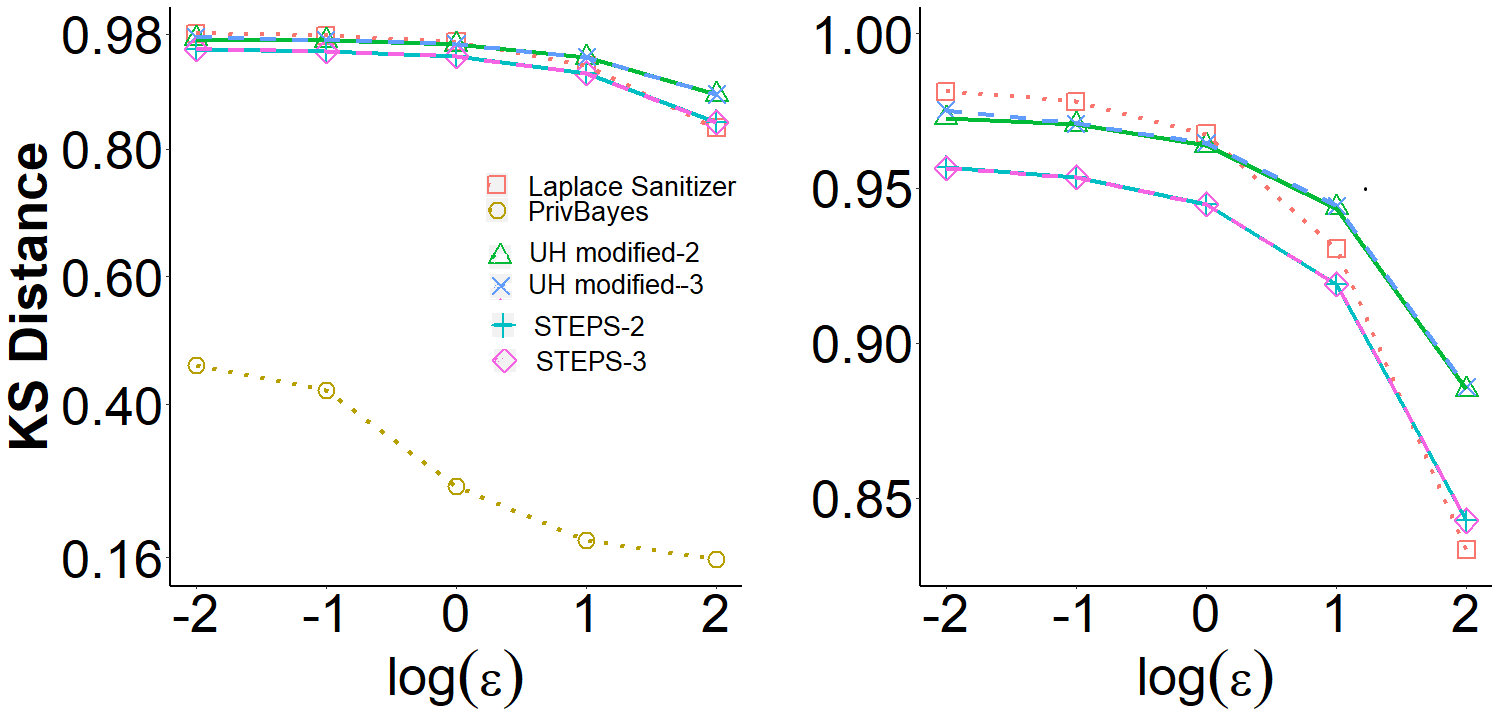
\includegraphics[scale=0.35]{SPECKS2.png}}
\vspace{-6pt}\caption{SPECKS analysis on the flat Laplace sanitizer, PrivBayes, STEPS, and a modified universal histogram with random partition. The plot on the left presents all the methods and the one on the right excludes PrivBayes} \label{fig:SPECKS}
\end{figure}
For all methods, the KS distance decreases as $\epsilon$ increases as expected, since the synthetic data are supposed to become closer to the actual data with more privacy budget. This expected trend also provides empirical evidence that SPECKS does what it is supposed to measure. Overall, PrivBayes outperforms all of the other methods for all levels of $\epsilon$. STEPS-2 and STEPS-3 are very similar and outperform the flat Laplace sanitizer (until $\log(\epsilon)=2$) and the UH modified-2 and UH modified-3 methods. The UH modified methods are similar to the flat Laplace sanitizer until around $\log(\epsilon)=2$. 

\subsubsection{Chi-squared tests of association}\label{sec:chi}
We conducted the chi-squared test of association for all possible 2-way tables (105 in total) across the 15 attributes to see how well the  statistically significant 2-way associations among the attributes in the original data are preserved in the synthetic data. Since the goal here is not to report which associations are statistically significant across all 105 tables, there is no need for multiplicity adjustment. We obtained the p-values from the chi-squared tests of association for all possible 2-way tables in each synthetic set and combined the p-values across the 5 synthetic sets via the combination rules from \citet{li1991significance}. 

\begin{figure}[!htb]
\centerline{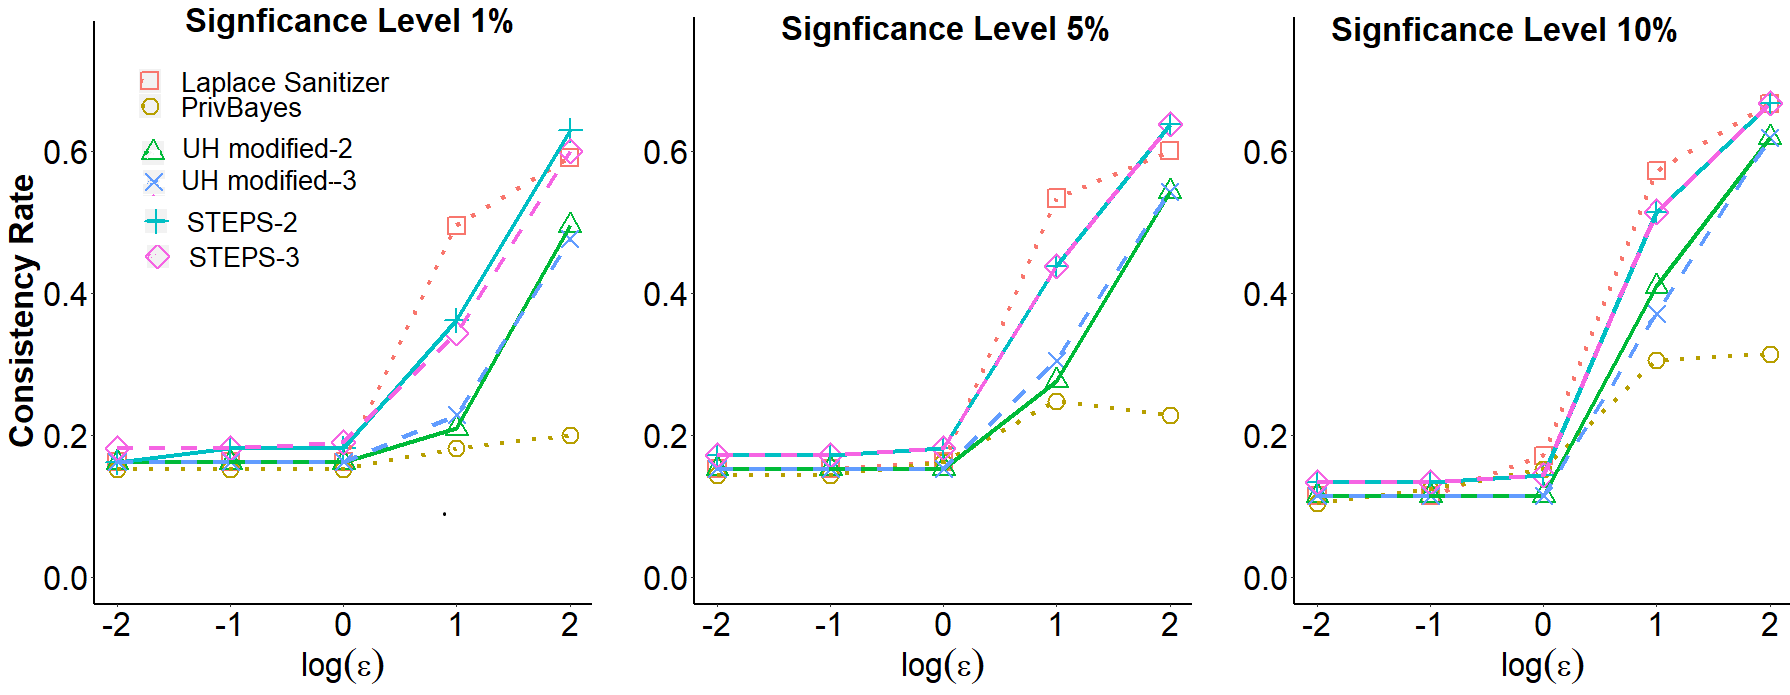
\includegraphics[width=6in]{accuracy2.png}}\vspace{-6pt}
\caption{Consistency rate on the statistical significance in the Chi-square test of association between the original and the synthetic data generated from the flat Laplace sanitizer, PrivBayes, STEPS, and a modified universal histogram with random partition.} \label{fig:chisq}\vspace{-6pt}
\end{figure}

Figure \ref{fig:chisq} presents the consistency rate, the percentage that the test conclusions are consistent between the original and synthetic data out of 105 tests) at the significance levels of $\alpha=\{1, 5, 10\}\%$, respectively. For most values of $\epsilon$, Laplace sanitizer and the STEPS methods outperform PrivBayes and the UH modified methods. At $\log(\epsilon) = 1$, the Laplace sanitizer has a higher consistency rate the STEPS methods; when $\log(\epsilon) = 2$, either the STEPS method performs better or performs similarly to the Laplace sanitizer. The UH modified methods also have a higher consistency rate on average than PrivBayes except for when $\log(\epsilon) = 0$ and $\alpha=\{0.05,0.10\}$.

%----------------------------------
\subsubsection{Difference-in-differences (DID) model}\label{sec:did}
We ran the DID model as conducted by \citet{Holbein2016} to examine the effects of ``Preregistration State'' on ``Voted'', controlling for ``Registration Status''. In the DID logistic regression model, the outcome is ``Vote'' with all the other 14 attributes as predictors plus an interaction term between ``Preregistration State'' and ``Registration Status''. ``Age'' is treated  as a numerical predictor whereas the others are categorical, leading to a total of 32 regression coefficients, including the intercept. We present the results using the confidence interval (CI) overlap approach by \citet{karr2006framework}, which measures how much the CIs for an coefficient of the same regression model obtained from the original data and the synthetic data overlap. The CI overlap value is between 0 and 1. A value of one corresponds to perfect match between the CIs based on the synthetic and original data (that is, the two CIs are identical), which is unlikely to achieve. A value of zero means there is no overlap between the two CIs. When one CI is completely contained within the other, the CI overlap value is greater than 0.5.

Figure \ref{fig:DID} shows the results for the average CIs across all 32 coefficients, ``Preregistration State'', ``Registration Status'', and the interaction term between ``Preregistration State'' and ``Registration Status'' (Prereg. x Reg.); the last three covariates are of primary interest in the DID model of \citet{Holbein2016}. 

\begin{figure}[!htb]
\centerline{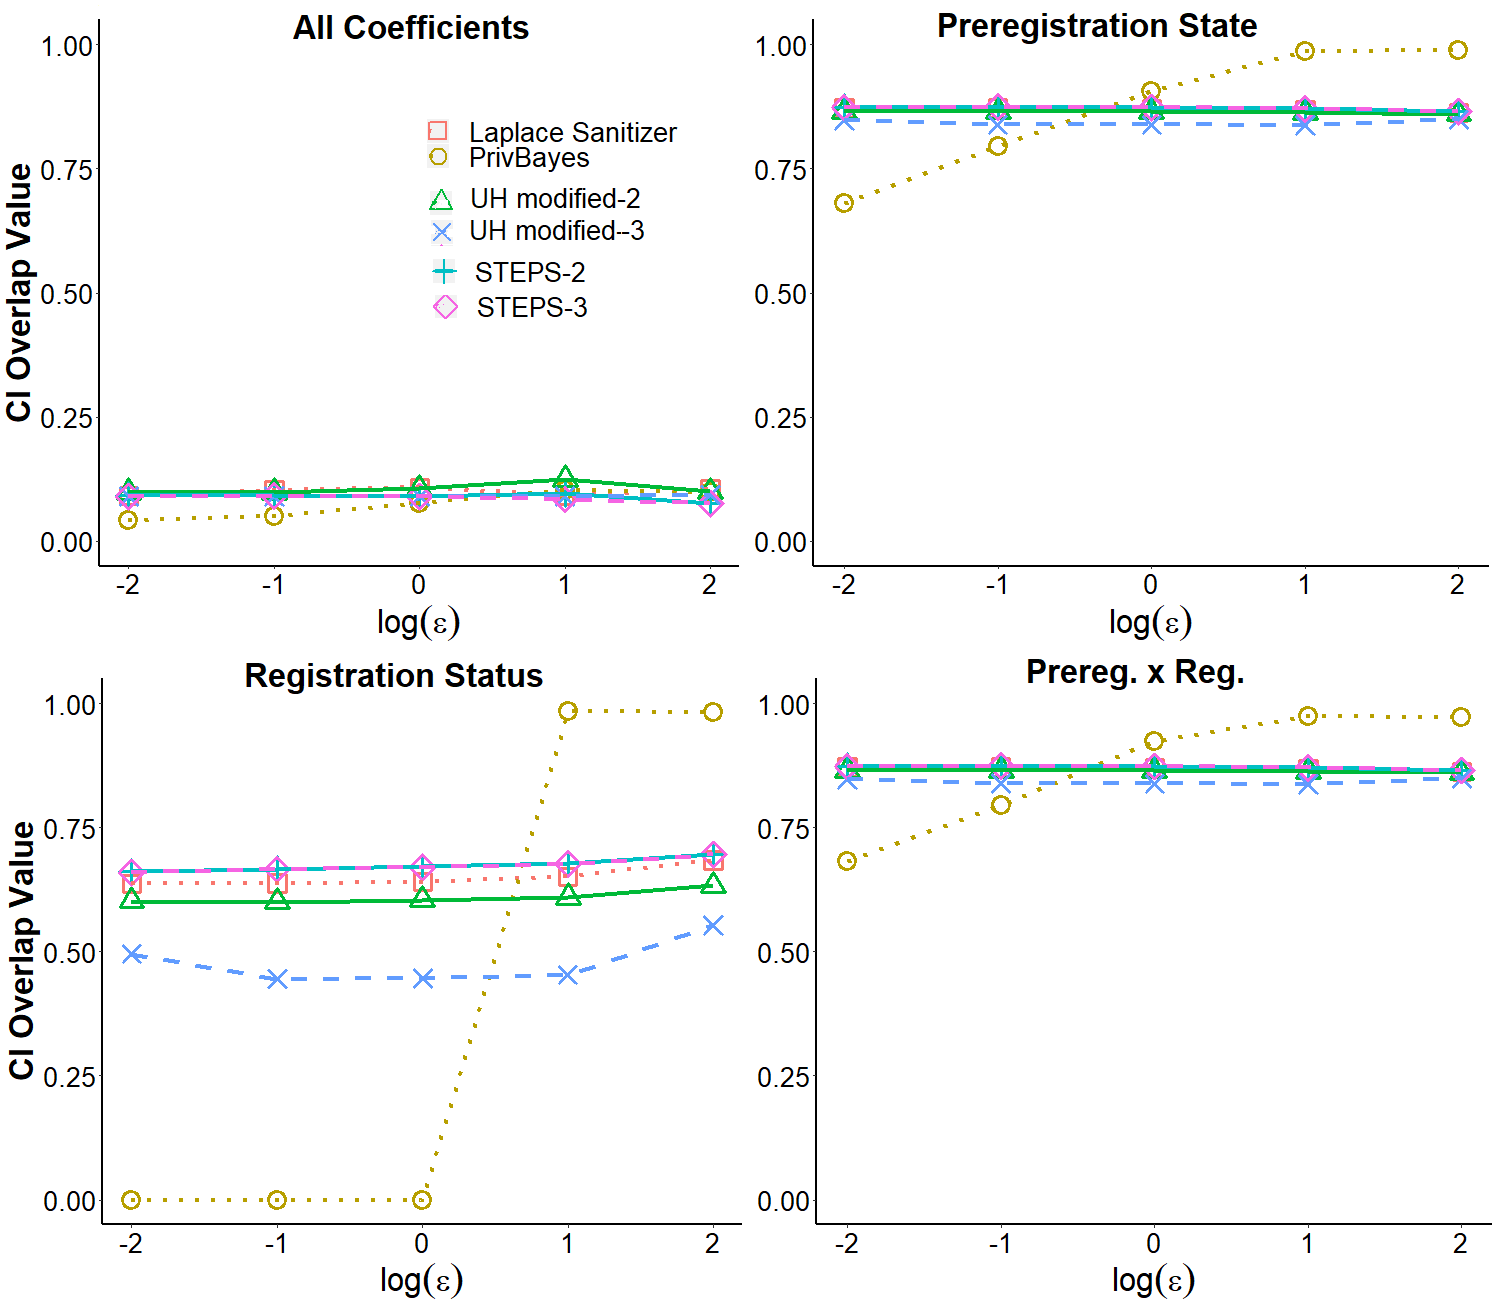
\includegraphics[width=5in]{DID2.png}}
\vspace{-6pt}\caption{Confidence interval (CI) overlap value analysis averaged across the 32 regression coefficients from the DID model fitted to the synthetic data generated from the flat Laplace sanitizer, PrivBayes, STEPS, and a modified universal histogram with random partition.} \label{fig:DID}
\end{figure}

For the average CI overlap value across the 32 coefficients, the methods performed poorly at all levels of $\epsilon$, because a big proportion of the 32 coefficients have a CI overlap value of close 0. The CI overlap values for the 3 covariates of interest are around 0.75 or above in most cases, suggesting good agreement between the CIs based on the synthetic data and on the original data. Among the four DIPS methods, PrivBayes has the lowest CI overlap values when $\log(\epsilon) < 0$. At higher levels of $\epsilon$, PrivBayes performed better with values closer to 1. The other methods remained flat across all levels of $\epsilon$. STEPS-2 and STEPS-3 performed similarly and had slightly higher values than the Laplace sanitizer whereas UH modified methods had the slightly smaller CI overlap values in general.

%--------------------------------------------------------
\section{Concluding Remarks}\label{sec:disc}

We propose the STEPS procedure to synthesize differentially private individual-level data. We also develop a propensity-based general utility metric, SPECKS, for assessing the similarity between the original and synthetic data. The STEPS method leverages the inherent information in the data to determine the partitioning order among the attributes. The sanitized counts of the nodes closer to the root of the tree (low-order marginals) have smaller mean squared errors than the nodes further away from the root because the former are weighted averages of more nodes. STEPS therefore preserves the information on more important attributes better than on less important ones, where the importance is determined either practically per domain knowledge or statistically. The STEPS procedure outperformed the modified universal histogram in general as it leverages the data to determine the partitioning sequence. Compared to PrivBayes and flat Laplace sanitizer, STEPS can preserve better either the population-level and the original information on a case-by-case basis.

We used the PrivBayes codes on GitHub at \citet{DataSynthesizercodes} developed by \citet{DataSynthesizer}. We noticed during the implementation that we needed to set a random seed in each synthetic generate; otherwise, every synthetic set is the same for a given $\epsilon$. Users of the codes need to keep that in mind when generating multiple synthetic sets to measure the synthesis uncertainty. Problems arising from implementing differentially private mechanisms and data synthesis methods are not new. \citet{kifer2020guidelines} describe the challenges as being a lack of a more robust framework and proper testing to prevent future difficulties in developing and publishing new differentially private methods. The authors encourage that every DP mechanism provides an accompanying mathematical proof on DP (not a just reference to the literature) along with proper code review and computational-aided verification/testing tools to avoid ``published mechanisms [that] do not satisfy differential privacy for any $\epsilon$ due to errors''.

For future work, we will look into developing general recommendations on the privacy budget allocation scheme between building the tree and sanitizing node counts, and among the layers. In addition, we will investigate the feasibility from the utility and computational prospective of developing a stopping rule on the tree height instead of pre-specifying the number of layers. For example, if the negative AIC is used the utility score for the exponential mechanism, we could examine the range of AIC from the marginal log-linear models with each of the available attributes at a node. If the range is within a certain threshold (say, 10\%), then the node will stop splitting and the full-dimensional histogram of the remaining attributes in that node will be constructed. Finally,
given that there are other propensity-score based general utility measures, we plan to compare SPECKS with those metrics via comprehensive empirical studies.

\section*{Acknowledgement}
We thank Madeline Brown, a Policy Assistant, at the Urban Institute for her expert knowledge in selecting variable order as a domain expert in the case study.

\bibliographystyle{agsm}
\setlength{\bibhang}{0pt}
\bibliography{reflist}

\end{document} 